\documentclass[t, pdftex]{beamer}
\usetheme[]{Cockrell}
%\usetheme[dept=Mechanical\ Engineering]{cockrell}

% \useoutertheme[subsection=false]{miniframes}
% \useoutertheme[footline=authortitle]{miniframes}
% \setbeamercolor{mini frame}{fg=white,bg=utblack}
%\usepackage{etoolbox}
%\patchcmd{\sectionentry}{\usebeamercolor[fg]{section in head/foot}}{\usebeamercolor[fg]{mini frame}}{}{}

\mode<presentation> {	
	% The Beamer class comes with a number of default slide themes	
	% which change the colors and layouts of slides. Below this is a list	
	% of all the themes, uncomment each in turn to see what they look like.
	
		
	%\usetheme{default}	
	%\usetheme{AnnArbor}	
	%\usetheme{Antibes}	
	%\usetheme{Bergen}	
	%\usetheme{Berkeley}	
	%\usetheme{Berlin}	
	%\usetheme{Boadilla}	
	%\usetheme{CambridgeUS}	
	%\usetheme{Copenhagen}	
	%\usetheme{Darmstadt}	
	%\usetheme{Dresden}	
	%\usetheme{Frankfurt}	
	%\usetheme{Goettingen}	
	%\usetheme{Hannover}	
	%\usetheme{Ilmenau}	
	%\usetheme{JuanLesPins}	
	%\usetheme{Luebeck}	
	%\usetheme{Madrid}	
	%\usetheme{Malmoe}	
	%\usetheme{Marburg}	
	%\usetheme{Montpellier}	
	%\usetheme{PaloAlto}	
	%\usetheme{Pittsburgh}	
	%\usetheme{Rochester}	
	%\usetheme{Singapore}	
	%\usetheme{Szeged}	
	%\usetheme{Warsaw}	
	
	% As well as themes, the Beamer class has a number of color themes	
	% for any slide theme. Uncomment each of these in turn to see how it	
	% changes the colors of your current slide theme.
	
	%\usecolortheme{albatross}	
	%\usecolortheme{beaver}	
	%\usecolortheme{beetle}	
	%\usecolortheme{crane}	
	%\usecolortheme{dolphin}	
	\usecolortheme{dove}	
	%\usecolortheme{fly}	
	%\usecolortheme{lily}	
	%\usecolortheme{orchid}	
	%\usecolortheme{rose}	
	%\usecolortheme{seagull}	
	%\usecolortheme{seahorse}	
	%\usecolortheme{whale}	
	%\usecolortheme{wolverine}
	
		
	\setbeamertemplate{footline} % To remove the footer line in all slides uncomment this line	
	%\setbeamertemplate{footline}[page number] % To replace the footer line in all slides with a simple slide count uncomment this line	
	
	%\setbeamertemplate{navigation symbols}{} % To remove the navigation symbols from the bottom of all slides uncomment this line
    
    \setbeamertemplate{itemize item}{\color{utblack}$\blacktriangleright$}
}

% Additional Settings
% From:
% https://tex.stackexchange.com/questions/37127/how-to-remove-some-pages-from-the-navigation-bullets-in-beamer/45038#45038
\makeatletter
\let\beamer@writeslidentry@miniframeson=\beamer@writeslidentry
\def\beamer@writeslidentry@miniframesoff{%
    \expandafter\beamer@ifempty\expandafter{\beamer@framestartpage}{}% does not happen normally
    {%else
        % removed \addtocontents commands
        \clearpage\beamer@notesactions%
    }
}
\newcommand*{\miniframeson}{\let\beamer@writeslidentry=\beamer@writeslidentry@miniframeson}
\newcommand*{\miniframesoff}{\let\beamer@writeslidentry=\beamer@writeslidentry@miniframesoff}
\makeatother

\addtobeamertemplate{navigation symbols}{}{%
	\usebeamerfont{footline}%
	\usebeamercolor[fg]{footline}%
	\hspace{1em}%
	\insertframenumber/\inserttotalframenumber
}

% Additional packages
\usepackage[]{algorithm}
\usepackage{algorithmic}
\usepackage{multicol}
% \usepackage{subfig}
\usepackage[english]{babel}
\usepackage{blindtext}
\usepackage{color}
\usepackage{cancel}
% \usepackage[]{algorithm2e}
\usepackage{mathtools}
\usepackage{amsmath}
\usepackage{pgfgantt}
\usepackage[version=3]{mhchem} % Package for chemical equation typesetting \ce{}
\usepackage{siunitx} % Provides the \SI{}{} and \si{} and \number{}
\newcolumntype{B}{>{\centering\arraybackslash}m{3cm}}
\newcolumntype{C}{>{\centering\arraybackslash}m{2cm}}
\newcolumntype{M}{>{\centering\arraybackslash}m{1.2cm}}
\newcolumntype{L}{>{\arraybackslash}m{8cm}}

\renewcommand{\CancelColor}{\color{utorange}}

% Additional Graphics Paths
\graphicspath{{./figs/}{../../../}{./}}

% Custom symbols and operators
\DeclareMathOperator*{\E}{\mathbb{E}}

% Bibliography definition
% \bibliography{../../dissertation/sections/refs.bib}
% \usepackage[hyperref=true,style=verbose,labeldate=true,minnames=2,maxnames=10,maxbibnames=99,backend=biber]{biblatex}
%\usepackage[backend=bibtex]{biblatex}
%\usepackage[backend=bibtex,sorting=none,hyperref=true,style=nature,isbn=false,doi=false,eprint=false,url=false]{biblatex}
\footnotesize{\bibliography{refs}}
%\setbeamerfont{bibliography entry author}{size=\small}
%\setbeamerfont{bibliography entry title}{size=\small}
%\setbeamerfont{bibliography entry location}{size=\small}
%\setbeamerfont{bibliography entry note}{size=\small}
%\setbeamerfont{bibliography item}{size=\small}
%\setbeamertemplate{footline}{%
%    \hfill \insertframenumber{} / \inserttotalframenumber \hfill \vspace*{1mm}
%}
\setbeamersize{text margin left=14pt, text margin right=14pt} %new code


\title{A CFD-Informed Hi2Lo Method for Subchannel Resolution Crud Prediction}
\subtitle{}
\author{William Gurecky}
\date{\today}


\begin{document}
\setbeamertemplate{caption}{\raggedright\insertcaption\par}
\setbeamertemplate{caption}{%
\begin{beamercolorbox}[wd=.5\paperwidth, sep=.2ex]{block body}\insertcaption%
\end{beamercolorbox}%
}

% =========================================================================== %
\titleframe
\frame{\frametitle{Outline}\tableofcontents}

% =========================================================================== %
\section{Introduction}
\subsection*{Crud Background}
\begin{frame}
\frametitle{Chalk River Unidentified Deposit (crud)}
\vspace{-12pt}
\begin{scriptsize}
    \begin{itemize}
     \item Deposited on rod surface where temperature is high - near or above saturation point - and where local shear stresses are low.
     \item Uptakes boron from the coolant driving
     crud induced power shift (CIPS).

	\item Crud can increase oxide ingress rates in certain zirc alloys leading to crud induced local corrosion (CILC) \cite{kendrick13}.

    \item CASL developed crud simulation package, MAMBA, which is integrated with the VERA core simulator \cite{collins16}.  
    \end{itemize}
\end{scriptsize}

\vspace{-12pt}
    \begin{figure}
        \centering
        \begin{minipage}{.5\textwidth}
            \centering
            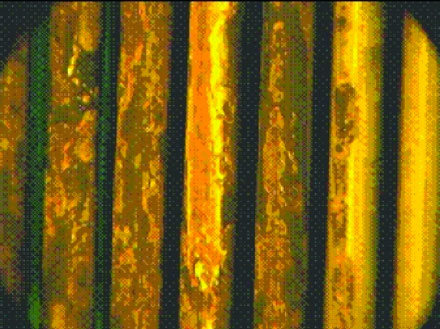
\includegraphics[width=0.55\textwidth]{figs/crud-crud.jpg}
        \end{minipage}%
        \begin{minipage}{.5\textwidth}
            \centering
            \includegraphics[width=0.55\textwidth]{figs/crud_flake_ex.png}
        \end{minipage}
    \end{figure}
\end{frame}

\begin{frame}
\frametitle{Chalk River Unidentified Deposit (crud)}
\vspace{-12pt}
\begin{scriptsize}
    \begin{itemize}
        \item Deposited on rod surface where temperature is high - near or above saturation point - and where local shear stresses are low.
        \item Crud uptakes and retains boron from the coolant which drives
        crud induced power shift (CIPS).       
        \[
        \frac{d N_{\mathrm{\ce{NiFe}},c}}{dt} = (\alpha_{\mathrm{nb}} + \alpha_{b}q''_{b} )N_{\mathrm{\ce{NiFe}}, \mathrm{cool}} - \gamma_k k
        \]
        \item $N_{NiFe,c}$: concentration of \ce{NiFe_2O_4}. $N_{NiFe,cool}$: concentration of nickel and iron particulates in the coolant.  $k$: near-cladding surface turbulent kinetic energy (TKE).  $q''$: boiling heat flux (nonzero at $T_s>T_{sat}$).  $\alpha_{nb}$: non-boiling coefficient. $\alpha_b$: boiling rate constant.  $\gamma_k$: erosion multiplier \cite{mongoose17}.
        
    \end{itemize}
\end{scriptsize}

\vspace{-12pt}
\begin{figure}
    \centering
    \begin{minipage}{.5\textwidth}
        \centering
        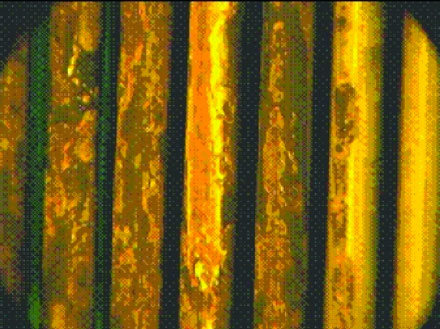
\includegraphics[width=0.55\textwidth]{figs/crud-crud.jpg}
    \end{minipage}%
    \begin{minipage}{.5\textwidth}
        \centering
        \includegraphics[width=0.55\textwidth]{figs/crud_flake_ex.png}
    \end{minipage}
\end{figure}
\end{frame}

% =========================================================================== %
\subsection*{Motivation}
\begin{frame}
    \frametitle{Crud Induced Power Shift (CIPS)}
    \vspace{-22pt}
    \begin{figure}
        \centering
        \begin{minipage}{.5\textwidth}
            \centering
            \includegraphics[width=6cm]{figs/ao_mpact_ctf.png}
            \caption{Core averaged \% axial offset.}
        \end{minipage}%
        \begin{minipage}{.5\textwidth}
            \centering
            \includegraphics[width=6cm]{figs/core_b10_mpact_ctf.png}
            \caption{VERA WBNP1 Cycle 7 crud \ce{^{10}B}. \\ $@ 16.08 [MWD/MTU]$}
        \end{minipage}
    \end{figure}
 \cite{collins2015}
\end{frame}

% =========================================================================== %
\subsection*{Motivation}
\begin{frame}
\frametitle{Crud Impacts on Industry}
\vspace{-24pt}
\begin{itemize}
    \item CIPS influences the burnup distribution reducing overall fuel utilization and can reduce shutdown margin  \cite{lange2017}.
    \item Plants seeking power uprates or lifetime extensions must prove the facility can operate within thermal limits.  Crud can complicate the analysis by shifting the power distribution and influencing surface heat transfer behavior which must be accounted for in DNB computations.
    \item Though rare, CILC failures require impacted assemblies to drastically reduce power and miss their burnup target.
    \item Crud ultrasonic/chemical shock treatment is an extra step to perform during reloading operations, costing time and potentially increasing radiation exposure risk to plant workers.
\end{itemize}
\textbf{Goal: Provide predictive capability to avoid CIPS limited fuel loading patterns.}
\end{frame}

% =========================================================================== %
\subsection*{Motivation}
\begin{frame}
\frametitle{Current Crud Model Deficiencies}
\begin{itemize}
    \item \textbf{Incorrect boundary conditions provided to the crud code.}
    \begin{itemize}
        \item Fine scale flow details around spacer grids are not resolved by subchannel codes.  It is imperative for CILC analysis to capture the influence of the spacer grids on the crud deposition rate.  
        \item It is also important to account for the presence of spacer grids on crud growth when predicting CIPS.
    \end{itemize}
    \item Incorrect simulated crud chemistry, pore fill mechanisms, and intra-crud species transport models.
    \item Difficulty accounting for the source of corrosion products and nickel and iron particulate entrained in the primary coolant loop.
    \begin{itemize}
        \item Requires understanding of the metallurgy of all primary loop components. 
        \item Plants of different make and vintage require a predictive corrosion and erosion source term models.
    \end{itemize}
\end{itemize}
\end{frame}


% =========================================================================== %
\subsection*{Hi2lo Overview}
\begin{frame}
\frametitle{Hi2lo}
\begin{figure}[]
    \vspace{-16.5pt}
    \centering
    \includegraphics[width=0.99\textwidth]{figs/mamba_hi2lo_vera_2.png}
    \label{hi2lo_overview}
\end{figure}
\vspace{-16.5pt}
\begin{itemize}
    \item Information flows from high fidelity (CFD) to low fidelity model (CTF) in a unidirectional manner.
    \item Hi2lo augments CTF solution to provide increased fidelity cladding surface temperature, near-wall TKE, and boundary heat flux estimates to MAMBA.
\end{itemize}
\end{frame}


% =========================================================================== %
\subsection*{State of Hi2lo}
\begin{frame}[shrink=10]
\frametitle{Prior Hil2o Work: HTC Spatial Remapping Procedure}
\begin{columns}
    \begin{column}{0.5\textwidth}
        \begin{itemize}
            \item Procedure based on mapping and re-scaling CFD results onto an intermediate reconstruction grid upon which crud is grown.
            \item The single phase heat transfer coefficient (HTC) and TKE surface fields are mapped.
            \item An iterative method is used to converge on the correct pin surface temperature given HTC and the boundary heat flux provided by CTF.
        \end{itemize}
    \end{column}
    \begin{column}{0.5\textwidth}  %%<--- here
        \begin{center}
            \begin{figure}
                \includegraphics[width=6cm]{figs/cfd_ctf_multi_grid.png}
                \caption{\centering TKE remapping procedure. \cite{salko17}}      
            \end{figure}
        \end{center}
    \end{column}
\end{columns}
\vspace{-12pt}
\end{frame}

% =========================================================================== %
\subsection*{State of Hi2lo}
\begin{frame}
\frametitle{Prior Hil2o Work: HTC Spatial Remapping Procedure}
\begin{figure}[!htbp]
\centering
\begin{minipage}{.5\textwidth}
    %
    \includegraphics[width=5cm]{figs/ctf_crud_orig.png}
    \caption{\centering \scriptsize{ Crud growth on the rod surface \\ prior to HTC and TKE \\ field remapping.}}
    \label{fig:crud_pre_map}
\end{minipage}%
\begin{minipage}{.5\textwidth}
    %
    \vspace{-5pt}
    \includegraphics[width=4.9cm]{figs/ctf_crud_reconstructed.png}
    \caption{\centering \scriptsize Crud growth on the rod \\ surface post HTC and TKE \\ field remapping.}
    \label{fig:crud_post_map}
\end{minipage}
\end{figure}
\cite{salko17}
\end{frame}

% =========================================================================== %
\subsection*{High Fidelity Crud Simulation}
\begin{frame}
\frametitle{Coupled CFD/Crud Calculation}
\vspace{-18pt}
\scriptsize{
    \begin{itemize}
    \item CFD/Crud coupling is useful for single-pin or single-assembly crud estimates.
    % Fine scale flow near spacer grid impacted surface crud distribution.  Important for quantifying crud induced local corrosion (CILC) risk.
    \item Too numerically costly for full core simulation.
    \end{itemize}
}
\begin{figure}[]
\centering
\includegraphics[width=0.95\textwidth]{figs/combo_180x.png}
\label{cfd_crud}
\end{figure}
\cite{slattery16}
\end{frame}

% =========================================================================== %
\subsection*{CFD and Subchannel Mesh Background}
\begin{frame}
\frametitle{CTF (subchannel) and CFD Meshes for a Single Pin}
\vspace{-20pt}
\begin{figure}
        \centering
        \begin{minipage}{.4\textwidth}
            \centering
            \includegraphics[width=3cm]{figs/cfd_ctf_mesh_v.png}
            \caption{\centering \scriptsize CTF (top).  CFD (bottom) }
        \end{minipage}%
        \begin{minipage}{.4\textwidth}
            \centering
            \includegraphics[width=2cm]{figs/ctf_mesh_v.png}
        \end{minipage}
\end{figure}
\cite{salko17}
\end{frame}

% =========================================================================== %
\subsection*{Crud State vs Thermal Hydraulic Surface Conditions Covariance Structure}
\begin{frame}
\begin{figure}[]
    \vspace{-16.5pt}
    \centering
    \includegraphics[width=10.88cm]{figs/ctf_patch_ex3_b.png}
    \label{model_overview}
\end{figure}
\end{frame}

% =========================================================================== %
\subsection*{CFD vs Subchannel:  Influcene on crud predictive capability}
\begin{frame}
On a single coarse CTF patch:
\vspace{-6.5pt}
\begin{figure}[!htbp]
    \centering
    \includegraphics[width=11cm]{figs/model_relations_2.png}
    \label{model_overview}
\end{figure}
\end{frame}

\section{Approach}
% =========================================================================== %
\begin{frame}\frametitle{Objectives}
\begin{itemize}
    \item Account for fine scale flow features unresolved by CTF on the growth of crud and boron hideout. \\

    \item Predict likelihood of temperatures in excess of saturation occurring in coincidence with low local turbulent kinetic energy. \\
    
    \item Preserve correlations between surface temperature, boundary heat flux and turbulent kinetic energy.
\end{itemize}
\end{frame}

% =========================================================================== %
\begin{frame}\frametitle{Approach}
\begin{itemize}
\item Forgo attempting to capture spatial intra-CTF patch distributions of temperature, boundary heat flux and TKE on rod surface. 
\item Track joint probability density, $f(T, TKE, q'')$, tallied over coarse CTF patches.
    \item Utilize a suite of precomputed CFD solutions to improve crud predictions given on the CTF grid. 
    \item Augment the CTF solution with a predicted stochastic component.
    \begin{itemize}
        \item CTF estimates mean TH conditions at a low spatial resolution.  
        \item The surrogate provides higher order moments about the mean.
    \end{itemize}
\end{itemize}
\end{frame}


% =========================================================================== %
\begin{frame}
    \frametitle{Approach}
    \vspace{-8pt}
    \begin{itemize}
    \item CTF estimates mean TH conditions at a low spatial resolution.  The surrogate provides higher order moments about the mean.
    
    \begin{block}{Rod Surface Field}
        \[ 
        F(\mathbf z) = \underbrace{\mu(\mathbf{z})}_\text{CTF} + \underbrace{\varepsilon(\mathbf z, {\mathbf p(\mathbf z)}) + b(\mathbf{z}) }_\text{CFD Informed}
        \]
    \end{block}
    \item Treat $\varepsilon$ as a random field.  $\varepsilon(\cdot)$ is a CFD informed model. $\mathbf z$ are spatial coordinates. $\mathbf p$ are a set of auxiliary predictors. \\
    \item $b$ is bias ($\mu_{CTF} - \mu_{CFD}$) \\
    $\mu$ is piecewise constant over each CTF patch
\end{itemize}
\end{frame}

% =========================================================================== %
\section[Theory]{Theory}
\subsection*{Problem Statement}
\begin{frame}
\textbf{Goal:} Compute the total integrated crud over a CTF patch with area $A$, for a single time step of $\delta t$.
\begin{itemize}
	\item Expected total crud over patch : 
	\begin{eqnarray}
		A \mu_g\ [grams] = A \E[\mathcal G(\mathbf x|\mathcal G_o, \mathbf I, \delta t)] \nonumber \\
		= A \iiint \mathcal G(\mathbf x|\mathcal G_o, \mathbf I, \delta t) h(\mathbf x|\theta) d \mathbf x  \nonumber
	\end{eqnarray}
	let $\mathbf x= \{T, k, q''\}$.
	$\mathbf I$ represents additional crud parameters, $\mathcal G_o$ is the crud state at the start of the time step and $\theta$ are distribution parameters.
	\item Estimate this integral via Monte Carlo:
	\[
	\E[g(x)] \approx \frac{1}{N} \sum_i^N \frac{\mathcal G(\mathbf x_i) 
	h(\mathbf x_i | \theta)}{\tilde h(\mathbf x_i | \tilde \theta)}, \ \mathbf x \sim \tilde h
	\]
	Where $\tilde h$ is an importance distribution. 
    \item \textbf{Problem:} $h$ is trivariate and must be accurately predicted on all CTF faces
\end{itemize}
\end{frame}


% =========================================================================== %
\subsection*{Copula Theory}
\subsubsection*{Capturing Dependence Between Random Variables}
\begin{frame}
\frametitle{Capturing Dependence - Sklar's Theorem}
\vspace{-16.5pt}
\begin{itemize}
\item Let $T=Temperature,\ k=TKE,\ q''=BHF$.
\item Given joint CDF: $H$, w/ cumulative margins: $F_T=P[T < t] = \int_{-\infty}^{t}f(w)dw$
\[
H(T,k) = C(F_T, F_k)
\]
\[
c(u, v) = \frac{\partial^2 C(u, v)}{\partial u \partial v};\ u=F_T, v=F_k
\]
% \item  The copula PDF, $c(\cdot)$ describes dependence between two random variables.
\item  Has uniform marginal density distributions \cite{Nelsen2006}.
\item  Defined on the unit square $[0, 1]^2$ (in the bivariate case)
\item  Any joint PDF, $h(\cdot)$ can be decomposed as: \\
\[
h(T, k) = c(u, v |\theta_c)f(T|\theta_T)f(k|\theta_k)
\]
Where $\theta_c$ and $\theta_{T,k}$ are free copula and marginal model parameters respectively.
\end{itemize}
\end{frame}

% =========================================================================== %
\subsection*{Copula Properties}
\begin{frame}[noframenumbering]
\frametitle{Specifying Copula Parameters}
\begin{itemize}
    \item For Archimedean copula, Kendall's tau, $\rho_\tau$ is
    related to the copula's shape parameter by:
    \[
    \rho_\tau = 1 + 4 \int_0^1 \frac{\varphi(\theta_c,t)}{\varphi'(\theta_c, t)}dt
    \]
    Where $\varphi(\theta_c, t)$ is the copula's generator function and $\varphi'$ is the first derivative of the generator function with respect to $t$.
    \item  $\rho_\tau$ is one-to-one with $\int_0^1 \frac{\varphi(\theta_c,t)}{\varphi'(\theta_c, t)}dt$.
    \item \textbf{Goal:} Associate each CTF patch with a copula family (categorical response) and Kendall's tau (real-valued).
\end{itemize}
\cite{Nelsen2006}
\end{frame}

\subsection*{Setup}
\begin{frame}
% =========================================================================== %
\frametitle<1>{Simplifications}
\frametitle<2>{Problem Setup}
\frametitle<3>{Problem Setup}
% --------------------------------------------------------------------------- %

\only<1>{
\begin{itemize}
    \item Assume the boundary heat flux is uncorrelated with the surface temperature and TKE.
    \item Assume boundary heat flux follows a Dirac delta function centered at the value predicted by VERA/CTF on each CTF face, $j$.
    \[
    f_{q''} = \delta_{(j,ctf)}
    \]
    Which results in

\[
h(T, k, q'') = c(u, v |\theta_c)f(T|\theta_T)f(k|\theta_k) f_{q''}
\]
    Where $\theta_c$ and $\theta_{T,k}$ are free copula and marginal model parameters respectively.
\end{itemize}
}
% --------------------------------------------------------------------------- %
\only<2>{
\[
h(T, k, q'') = c(u, v |\theta_c)f(T|\theta_T)f(k|\theta_k) f_{q''}
\]
    \begin{itemize}
        \item Predict (denoted by $\hat{(\cdot)}$ notation):
        \begin{itemize}
            \item $\hat \theta_c$ and $\hat \theta_{T,k}$ on all CTF faces. 
        \end{itemize}  
        
        \item What functional form do the marginal and copula distributions take?
        
        \item By what method are the distribution parameters predicted?
    \end{itemize}
}
% --------------------------------------------------------------------------- %
\only<3>{
    \begin{itemize}
        \item It is necessary to predict (denoted by $\hat{(\cdot)}$ notation):
        \begin{itemize}
            \item $\hat \theta_c$ and $\hat \theta_{T,k}$ on all CTF faces. 
        \end{itemize}  
        
        \item What form do the marginal and copula distributions take?
        \begin{itemize}
            \item Adopt a non-parametric representation of the temperature and TKE marginal distribution on each CTF face.  The CFD born distributions do not conform to a known parametric distribution family and cannot be reliably transformed to be Gaussian-like since this transformation would vary from CTF face to face.
            \item Choose a copula from a library of parametric copula families via KL divergence or AIC based best-fitting metrics.
        \end{itemize}        
        \item By what method are the distribution parameters predicted?
        \begin{itemize}
            \item Gradient boosted quantile regression trees for $\hat \theta_{T,k}$.
            \item Gradient boosted regression trees for $\hat \theta_{c}$.
        \end{itemize}
    \end{itemize}
}
\end{frame}

% =========================================================================== %
\subsection*{Quantiles}
\begin{frame}
\frametitle{Representation of Margins: Sample Quantiles}
\vspace{-15pt}
    \begin{columns}
        \begin{column}{0.5\textwidth}
            \scriptsize{
                \begin{itemize}
                    \item Given a set of sample quantiles, $\hat{\mathbf{\theta}_T} = \{\hat q_{\tau_0}, \hat q_{\tau_i}, ... \hat{q}_{\tau_{N_Q}} \}$
                    \item The quantile function can be inverted to give the CDF:
                    \[
                    \hat F_T = \hat{Q}^{-1}(T; \mathbf{\hat \theta}_T)
                    \]
                    \item Piecewise linear CDF shown in figure results in histogram-like PDF.  The function is supported at the known nodes: $\{ \hat q_{\tau_0}, \hat q_{\tau_i}, ... \hat q_{\tau_{N_Q}} \}$
                    \item Where $N_{Q}$ is the number of quantiles we desire to retain in the reconstruction and is a user set runtime parameter.
                \end{itemize}
            }
        \end{column}
        \begin{column}{0.5\textwidth}  %%<--- here
            \begin{center}
                \includegraphics[width=0.9\textwidth]{figs/margins_cdf_2.png}
            \end{center}
        \end{column}
    \end{columns}
\end{frame}

% =========================================================================== %
%\subsection*{Gradient Boosting}
%\begin{frame}
%\begin{itemize}
% \item By what method are the distribution parameters predicted?
%\begin{itemize}
%    \item Gradient boosted quantile regression trees for $\hat \theta_{T,k}$.
%    \item Gradient boosted regression trees for $\hat \theta_{c}$.
%\end{itemize}
%\end{itemize}
%\end{frame}

% =========================================================================== %
\subsection*{Gradient Boosting}
\begin{frame}
\frametitle{Gradient Boosting}
\vspace{-8pt}
\begin{itemize}
    \item Supervised machine learning method for classification and regression
    \item Gradient descent in function space
    \item Find $\mathcal F_M$ that maps the inputs $\mathbf p$ to training data, $y$, where $\mathcal F_M$ is given by:
    \[
    \mathcal F_M = \text{argmin}_{\mathcal F} \E_{y, \mathbf p} [ L(y, \mathcal F(\mathbf p)) ]
    \]\\
    $L(\cdot)$: differentiable loss function.  $\mathbf p$: predictive features. $y$: response.  Paired set $\{\mathbf p, y \}$ is the \emph{training data set}.
%    \item Sum-of-trees ensemble technique:
%    \[
%    \mathcal F_M(\mathbf p, \mathbf{\gamma}, \mathbf b) = \sum_{m=0}^M \gamma_m h_m(\mathbf p; b_m)
%    \label{eq:single_cart_model}
%    \]
\begin{figure}[!htbp]
    \centering
    \includegraphics[width=0.65\textwidth]{figs/pseudo_resids.png}
    \label{model_overview}
\end{figure}
\end{itemize}
\cite{prett2014}
\end{frame}

% =========================================================================== %
\begin{frame}
\frametitle{Gradient Boosting}
\vspace{-8pt}
\begin{itemize}
    % \item Denote the gradient boosted model as $\mathcal F_M$.
    \item With the appropriate loss function, $L(\cdot)$, the gradient boosted model is trained to produce the conditional quantiles we seek:
    \[
     \hat{\mathcal F_M} =  \mathrm{argmin}_{\mathcal F}
     \E [ L(\mathcal{F}_M (\mathbf p), \theta(\mathbf p)) ]
    \]
    \item Supply local thermal hydraulic conditions, $\mathbf p_j$, near CTF face $j$ to evaluated the trained model:
    \[
    \hat \theta_j \leftarrow \hat{\mathcal F_M}(\mathbf p_j)
    \]
    \item  The boosted model is treated as a meta-model containing many independent predictors for each conditional quantile of interest.
    \[
    \ \ \hat \theta_j = \{\hat \theta_{j,c}, \hat \theta_{j,T}, \hat \theta_{j,k} \}
    \]
    % \item Covarience between quantiles is ignored in the current implementation of the boosted quantile regression models.
\end{itemize}
\cite{friedman2001}
\end{frame}

% =========================================================================== %
\subsection*{Gradient Boosting Quantile Regression Example}
\begin{frame}
\vspace{-18pt}
    \[
    y = x\ \mathrm{sin}(x) +12 \mathcal H(x-5)+\varepsilon; \ \ x\in [0,10]; \ \ \varepsilon \sim \mathcal N(0,2)
    \]
    \vspace{-10pt}
\scriptsize{
\begin{itemize}
    % \item $\mathcal H$ denotes the Heaviside function. 
    % \item Synthetic noise, $\varepsilon \sim \mathcal N(0,2)$ 
    \item 5000 total samples were drawn from the test function.  The test data was spatially aggregated to 100 axial levels to mimic CTF axial grid spacing.
    \item Quantile Loss minimized by gradient boosted model:
    \vspace{-4pt}
    \[
    L(y, \mathcal F(p);\tau) = \left[ (1-\tau) \sum_{y \leq \mathcal F(p)}( y_i - \mathcal F(p) ) \right] - \left[ \tau \sum_{y > \mathcal F(p)} (y_i - \mathcal F(p)) \right]
    \]
\end{itemize}   
}
\vspace{-26pt}
\begin{columns}
    \begin{column}{0.5\textwidth}
        \begin{figure}
            \centering
            \includegraphics[width=1.0\linewidth]{dissertation/figs/grad_boost/1d_boosted_regression_quantile_ex_0_5}
            \caption{\centering \scriptsize Median prediction over 80 trials.}
        \end{figure}
    \end{column}
    \begin{column}{0.5\textwidth}  %%<--- here
        \begin{figure}
            \centering
            \includegraphics[width=1.0\linewidth]{dissertation/figs/grad_boost/1d_boosted_regression_quantile_ex_0_95}
            \caption{\centering \scriptsize $\hat{q}_{\tau=0.95}$ prediction over 80 trials.}
        \end{figure}
    \end{column}
\end{columns}
\end{frame}

% =========================================================================== %
\begin{frame}
\vspace{-8pt}
\begin{itemize}
    \item Check to ensure quantile residuals (computed vs. expected) follow the expected theoretical behavior.
    \item Tested two different gradient boosting libraries.  ({\color{utblue} Custom implementation  (blue)}. {\color{utred} sk-learn (red)})
\end{itemize}
\vspace{-8pt}
%\begin{columns}
%    \begin{column}{0.5\textwidth}
%        \begin{figure}
%            \centering
%            \includegraphics[width=1.1\linewidth]{dissertation/figs/grad_boost/1d_boosted_regression_quantile_resid_0_5}
%            \caption{\centering \scriptsize Median residual distributions vs. theory.}
%        \end{figure}
%    \end{column}
%    \begin{column}{0.5\textwidth}  %%<--- here
%        \begin{figure}
%            \centering
%            \includegraphics[width=1.1\linewidth]{dissertation/figs/grad_boost/1d_boosted_regression_quantile_resid_0_95}\\
%            \caption{\centering \scriptsize $\tau=0.95$ residual distributions vs. theory.}
%        \end{figure}
%    \end{column}
%\end{columns}

\begin{figure}
    \centering
    \includegraphics[width=0.67\linewidth]{dissertation/figs/grad_boost/1d_boosted_regression_quantile_resid_0_95}\\
    \caption{\centering \scriptsize $\tau=0.95$ residual distributions vs. theory.}
\end{figure}
\end{frame}

\section[Synthetic Data]{Synthetic CFD Data Source for Model Validation}
% =========================================================================== %
\begin{frame}
\begin{itemize}
    \item Augment baseline CTF result by a user-specified bias, $\mathbf b$ and stochastic component, $\varepsilon(\mathbf z; \theta)$:
    \begin{align}
    \mathbf X &= \mathbf \mu_{ctf} + \mathbf b + \mathbf \varepsilon \nonumber \\
    &=
    \begin{pmatrix}
    T \\
    k \\
    q''
    \end{pmatrix}
    =
    \begin{pmatrix}
    \mu_{T} \\
    \mu_k \\
    \mu_{q''}
    \end{pmatrix}_{ctf}
    + \begin{pmatrix}
    b_{T} \\
    b_k \\
    b_{q''}
    \end{pmatrix}
    + \mathbf{\varepsilon} (\mathbf z; \mathbf \theta) \nonumber
    \end{align}
\end{itemize}
\end{frame}

\section[Applied Methods]{Applied Methods: Monte Carlo Crud Integration \& Propagating Crud Through Time}
% =========================================================================== %
\subsection*{Sampling}
\begin{frame}
\frametitle{Monte Carlo Sampling}
\vspace{-16pt}
\begin{itemize}
    \item Obtain $\ \ \hat \theta_j = \{\hat \theta_{j,c}, \hat \theta_{j,\{k, T\}} \}$ via evaluation of the gradient boosted model: $\hat \theta_j \leftarrow \hat{\mathcal F_M}(\mathbf p_j, \mathbf z_j)$.
    \item Drop understood patch index: $j$ 
    \item Define the reconstructed joint density as:
\begin{align}
h(T, k, q'') = & f_T(T;\hat \theta_T) f_k(k;\hat \theta_k) f_{q''} \cdot \nonumber \\
& c_{T,k}(F_T(T;\hat \theta_{T}),F_k(k;\hat \theta_{k});\hat \theta_c) \nonumber
\label{eq:joint_t_tke_q}
\end{align} 

\item Let:
\[ \mathbf X=\{T, k, q''\} \]

\item An estimate for the amount of crud on a given patch:
\begin{equation}
\E(\mathcal G(X)) \approx \frac{1}{N} \sum_i^N \mathcal G(X_i), \ \mathbf{X} \sim {h} \nonumber
\label{eq:mc_expected_crud}
\end{equation}
\end{itemize}
\end{frame}

% =========================================================================== %
\begin{frame}
\frametitle{\small Monte Carlo Sampling of the Joint Distribution over a Single Patch}
\vspace{-19pt}
\begin{figure}[!htbp]
    \centering
    \includegraphics[width=1.0\linewidth]{/dissertation/figs/imp_patch/original_t_tke_bmass_scatter_cut}
    \label{model_overview}
\end{figure}
\end{frame}

% =========================================================================== %
\begin{frame}
\frametitle{Importance Sampling}
\vspace{-16pt}
\begin{itemize}
    \item Specify a sampling (proposal) distribution, $\tilde h$.

\begin{equation}
\E(\mathcal G(X)) \approx \frac{1}{N} \sum_i^N \mathcal G(X_i) \frac{h(X_i)}{\tilde h(X_i)}, \ \mathbf{X} \sim \tilde{h} \nonumber
\label{eq:mc_imp_expected_crud}
\end{equation}

\item The sample importance is given by the ratio between the target and sampling distributions:
    
    \begin{equation}
    \omega_i = \frac{h_i}{\tilde h_i} = \frac{f_T(t_i) f_k(k_i)c(F_T(t_i), F_k(k_i))}{\tilde f_T(t_i) \tilde f_k(k_i) \tilde c(\tilde F_T(t_i), \tilde F_k(k_i))} \nonumber
    \label{eq:imp_prob_ratio}
    \end{equation}

    \item \textbf{Goal:}  Target regions of the rod surface which exhibit changes in crud behavior and contribute to crud growth: $T \ge T_{sat}$ and low TKE.  Avoid sampling heavily in regions with $T<T_{sat}$.
\end{itemize}
\end{frame}

% =========================================================================== %
\subsection*{Crud Boundary Condition Sensitivity}
\begin{frame}
\frametitle{Chalk River Unidentified Deposit (crud)}
\vspace{-12pt}
\begin{itemize}
    \item Crud boron deposition rate vs. surface temperature and TKE.
\end{itemize}
\begin{figure}
    \centering
    \begin{minipage}{.5\textwidth}
        \centering
        \includegraphics[width=1.01\linewidth]{/dissertation/figs/crud/crud_t_tke_boron_response_80}
        \caption{\centering Boundary heat flux: \\ $q''=80[W/cm^2]$.  }
    \end{minipage}%
    \begin{minipage}{.5\textwidth}
        \centering
        \includegraphics[width=1.01\linewidth]{/dissertation/figs/crud/crud_t_tke_boron_response_120}
        \caption{\centering  Boundary heat flux: \\ $q''=120[W/cm^2]$. }
    \end{minipage}
    pyMAMBA results. 
\end{figure}
\end{frame}

% =========================================================================== %
\subsection*{Importance Sampling}
\begin{frame}
\frametitle{\small Importance Sampling of the Joint Distribution over a Single Patch}
\vspace{-19pt}
\begin{figure}[!htbp]
    \centering
    \includegraphics[width=1.0\linewidth]{/dissertation/figs/imp_patch/importance_t_tke_bmass_scatter_cut}
    \label{model_overview}
\end{figure}
\end{frame}

% =========================================================================== %
\begin{frame}
\frametitle{Importance Sampling Distributions}

\begin{itemize}
    \item {\color{utred} Proposal (red)} vs. {\color{utblue} original (blue)} marginal distributions.
\end{itemize}
\vspace{-18pt}
\begin{columns}
    \begin{column}{0.5\textwidth}
\begin{figure}[]
\centering
\includegraphics[width=1.1\linewidth]{/dissertation/figs/imp_patch/temperature_importance_marginal_compare}
\caption{\centering Temperature}
\label{model_overview}
\end{figure}
\end{column}
\begin{column}{0.5\textwidth}
\begin{figure}[]
\centering
\includegraphics[width=1.1\linewidth]{/dissertation/figs/imp_patch/tke_importance_marginal_compare}\\
\caption{\centering TKE}
\label{model_overview}
\end{figure}
\end{column}
\end{columns}
\end{frame}

% =========================================================================== %
\begin{frame}
\frametitle{\small Importance Sampling Results on a Single Patch}
\vspace{-18pt}
\begin{itemize}
    \item Importance sampling trial results on a single CTF face. {\color{utred}Red} denotes importance samples and {\color{utblue}blue} denotes standard Monte Carlo samples.  
\end{itemize}
\[ \frac{\sigma^2_{MC}}{\sigma^2_{I}} \approx (\num{4.979e-6})^2 / (\num{3.503e-6})^2  \approx 2.02 \]
\vspace{-18pt}
%\begin{columns}
%    \begin{column}{0.5\textwidth}
%\begin{figure}[]
%    \centering
%    \includegraphics[width=1.0\linewidth]{/dissertation/figs/imp_patch/bmass_sample_violin}
%    \caption{\centering (a)}
%    \label{model_overview}
%\end{figure}
%\end{column}
%\begin{column}{0.5\textwidth}
%\begin{figure}[]
%    \centering
%    \includegraphics[width=1.0\linewidth]{/dissertation/figs/imp_patch/cmass_sample_violin}\\
%    \caption{\centering (b)}
%    \label{model_overview}
%\end{figure}
%\end{column}
%\end{columns}

\begin{figure}[]
    \centering
    \includegraphics[width=0.65\linewidth]{/dissertation/figs/imp_patch/cmass_sample_violin}\\
    \label{model_overview}
\end{figure}
\end{frame}


\subsection*{Time Stepping}
% =========================================================================== %
\begin{frame}
\frametitle{Propagating Crud Through Time}
\vspace{-16pt}
\begin{itemize}
    \item Thermal hydraulic state, including power distribution and flow rates, changes through a cycle.  
    \item Provide a mechanism to step the solution forward in time, akin to solving the following stochastic ODE:
    \[
    \frac{d N}{d t} = \alpha N - \gamma_k k
    \]
    Where $\alpha$ and $\gamma_k$ are random variables whose governing distributions depend on the local core state.
\end{itemize}

\begin{figure}[]
\centering
\includegraphics[width=0.9\linewidth]{figs/crud_time_demo.png}
\label{model_overview}
\end{figure}
\end{frame}


% =========================================================================== %
\begin{frame}[shrink=10]
\frametitle{Propagating Crud Through Time}
\begin{itemize}
\item  \textbf{Problem:}  The crud growth rate depends on the previous crud state. 
\end{itemize}
\begin{figure}[!htbp]
\centering
\begin{minipage}{.5\textwidth}
  \includegraphics[width=5cm]{figs/dboron_dt_tke.png}
\caption{\centering Crud growth rate TKE \\ sensitivity vs. Time. \\ $T=620[K], q''=100[W/cm^2]$.} 
\label{fig:crud_pre_map}
\end{minipage}%
\begin{minipage}{.5\textwidth}
  \includegraphics[width=5cm]{figs/dboron_dt_t.png}
\caption{\centering Crud growth rate Temperature \\ sensitivity vs. Time. \\ $TKE=0.01[J/kg], q''=100[W/cm^2]$..}
\label{fig:crud_post_map}
\end{minipage}
\end{figure}
\end{frame}

% =========================================================================== %
\begin{frame}[shrink=20]
\frametitle{Propagating Crud Through Time: Patch Remapping}
\begin{columns}
\begin{column}{0.5\textwidth}
    Two bounding cases to consider:
\scriptsize{
   
\begin{itemize}
\item Hot spots on the rod surface remain stationary w.r.t time
	\begin{itemize}
	\item Re-order samples such that the highest temperature sample always occurs in the same location inside a patch.
	\end{itemize}
\item Converse: Hot spots randomly move about the rod as time goes on
	\begin{itemize}
	\item Randomize samples inside a patch - do not preserve any spatial structure of the temperature distribution.
	\end{itemize}
\end{itemize}
Define a metric; for each $\mathcal F_i$ compute:
\[
    m_i = w_T \left( \frac{T_i - T_{min}}{T_{max} - T_{min}} \right) + w_k \left( \frac{k_i - k_{min}}{k_{max} - k_{min}} \right) +  w_q'' \left( \frac{q^{''}_i - q^{''}_{min}}{q_{max} - q_{min}} \right)
\]
Rank $m_i$ by highest to lowest with and store the ranked indices.
}
\end{column}
\begin{column}{0.5\textwidth}  %%<--- here
    \begin{center}
     \includegraphics[width=0.85\textwidth]{figs/sample_mapping.png}
     \end{center}
\end{column}
\end{columns}
\end{frame}

% =========================================================================== %
\begin{frame}[shrink=20]
\frametitle{\small Propagating Crud Through Time: With Importance Sample Weights}
\vspace{-20pt}
\begin{itemize}
    \item Define sample remapping:  $ \mathcal R $  
    \item Draw samples, $X \sim \tilde h$ and compute sample weights, $\mathbf \omega$.
    \item Remap samples:  $\mathbf x', \omega' \xleftarrow[\text{ }]{\mathcal R} \mathbf x, \omega $
    \item For $ i \in [0, 1, ... N]$  Where $N$ is the number of samples drawn per CTF Face:
\end{itemize}
\begin{columns}
    \begin{column}{0.5\textwidth}
Compute time averaged importance weights:
\begin{align}
\bar \omega'_{{n},i} &= \left( \frac{(n-1) \Delta t_s}{n \Delta t_s} \right) \bar \omega'_{n-1,i} + \left( \frac{\Delta t_s}{n \Delta t_s} \right) \omega'_{n,i} \nonumber \\
&= \left( \frac{(n-1)}{n} \right) \bar \omega'_{n-1,i} + \left( \frac{1}{n} \right) \omega'_{n,i} \nonumber
\label{eq:time_sample_weights3}
\end{align}
Where $n$ is the current resampling step index.
Crud growth step:
\[
\mathbf C_{n,i} = \mathcal G(x'_i; \mathbf C_{i, n-1}, \mathbf I, \Delta t_s)
\]
\begin{equation}
C_{m} = \left(\frac{A}{\sum_i^M \bar \omega'_i}\right) \sum_i^N C'_i \bar \omega'_i \nonumber
\label{eq:patch_sum_mass}
\end{equation}
   \end{column}
\begin{column}{0.5\textwidth}
\begin{figure}[H]
    \centering
    \includegraphics[width=0.9\linewidth]{/dissertation/figs/step_scheme}
    \caption{Multi-state point time stepping overview.  Multiple Resampling events are conducted per VERA state.  $\Delta t_s$ is a user controllable resampling step size parameter.}
    \label{fig:stepscheme}
\end{figure}
 \end{column}
\end{columns}
\end{frame}

% =========================================================================== %
\begin{frame}
\frametitle{Remap samples on a CTF Patch}
    \begin{figure}
        \centering
        \begin{minipage}{.5\textwidth}
            \centering
            \includegraphics[width=6cm]{figs/new/patch_rand_t_ex.png}
            \caption{\centering Randomized temperature \\ samples on a patch.}
        \end{minipage}%
        \begin{minipage}{.5\textwidth}
            \centering
            \includegraphics[width=6cm]{figs/new/patch_t_ex.png}
            \caption{\centering Re-ordered temperature samples. \\ $w_T=1.0; w_k=w_{q''}=0$}
        \end{minipage}
    \end{figure}
Both patches share the \emph{same} PDF of temperature, however, the spatial distributions are not equal.
\end{frame}

% =========================================================================== %
\begin{frame}
\frametitle{Remap samples on a CTF Patch}
    \begin{figure}
        \centering
        \begin{minipage}{.5\textwidth}
            \centering
            \includegraphics[width=6cm]{figs/new/patch_rand_tke_ex.png}
            \caption{\centering Randomized TKE \\  samples on a patch.}
        \end{minipage}%
        \begin{minipage}{.5\textwidth}
            \centering
            \includegraphics[width=6cm]{figs/new/patch_tke_ex.png}
            \caption{\centering Re-ordered TKE samples. \\  $w_T=1.0; w_k=w_{q''}=0$}
        \end{minipage}
    \end{figure}
Both patches share the \emph{same} PDF of TKE, however, the spatial distributions are not equal.
\end{frame}

% =========================================================================== %
\begin{frame}
\frametitle{Mapping strategy comparison: Single pin results}
\begin{itemize}
    \item Pin-integrated Boron inside the crud as a function of time.  
    \item {\color{utgreen} Green: Assumes randomly moving hot spots.} 
    \item {\color{blue} Blue: Assumes stationary hot spots ( $w_T=1.0; w_k=w_{q''}=0$).}
\end{itemize}

\vspace{-16pt}
\begin{figure}[!htbp]
\centering
\includegraphics[width=0.6\textwidth]{figs/new/cmpr_pin_totals.png}
\label{model_overview}
\end{figure}
\end{frame}


% =========================================================================== %
\begin{frame}
\frametitle{Single Pin Results: No Sample Remapping}
\vspace{-16pt}
\scriptsize{
\begin{itemize}
    \item No Sample Remapping Performed i.e:
    Ranked samples $\mathbf m'$ are randomly emplaced on the CTF faces.
    \item Hot spots are allowed to randomly move about the rod surface at each resampling step.
    \item Non-physical
\end{itemize}
}
\begin{figure}[!htbp]
    \centering
    \begin{minipage}{.5\textwidth}
        \includegraphics[width=1.1\linewidth]{figs/avg_method/cmpr_pin_totals.png}
        \caption{\centering Pin integrated crud boron \\ as a function of time.} 
        \label{fig:crud_pre_map}
    \end{minipage}%
    \begin{minipage}{.5\textwidth}
        \includegraphics[width=1.1\linewidth]{figs/avg_method/struct_pin_z_bmass.png}
        \caption{\centering Crud boron mass distribution at 300[days].}
        \label{fig:crud_post_map}
    \end{minipage}
\end{figure}
\end{frame}

% =========================================================================== %
\subsection*{Time Dependence}
\begin{frame}
\frametitle{Single Pin Results:  Remapping Applied}
\begin{itemize}
    \item Approximately optimal remapping coefficients: $w_T=0.4, w_k=0.6, w_{q''}=0$. 
\end{itemize}
    \begin{figure}
        \centering
        \begin{minipage}{.5\textwidth}
            \centering
            \includegraphics[width=6cm]{figs/map_method/cmpr_pin_totals.png}
            \caption{\centering Total rod crud boron vs. time.}
        \end{minipage}%
        \begin{minipage}{.5\textwidth}
            \centering
            \includegraphics[width=6cm]{figs/map_method/struct_pin_z_bmass.png}
            \caption{ \centering Crud Boron Deposition $[g/cm^2]$}
        \end{minipage}
    \end{figure} 
\end{frame}

% =========================================================================== %
\begin{frame}
\frametitle{Single Pin Results $@$ 300 days}
\begin{itemize}
    \item Approximately optimal remapping coefficients: $w_T=0.4, w_k=0.6, w_{q''}=0$. 
\end{itemize}
    \begin{figure}
        \centering
        \begin{minipage}{.5\textwidth}
            \centering
            \includegraphics[width=6cm]{figs/map_method/struct_pin_z_twall.png}
            \caption{\centering Axial cladding outer \\ surface temperature distribution [K].}
        \end{minipage}%
        \begin{minipage}{.5\textwidth}
            \centering
            \includegraphics[width=6cm]{figs/map_method/struct_pin_z_tke.png}
            \caption{ \centering Axial cladding outer \\ surface TKE distribution [J/kg]}
        \end{minipage}
    \end{figure}
\end{frame}


% =========================================================================== %
\subsection*{Hi2lo method for time dependent crud prediction}
\begin{frame}
\frametitle{Hi2lo Method Recap}
\vspace{-28pt}
\begin{columns}
     \vspace{22pt}
    \begin{column}{0.5\textwidth}
        
        Upfront:
        \begin{enumerate}
            \item Preprocess CFD data
            \item Train ML models
         \end{enumerate}
     \vspace{18pt}
        At Runtime:
         \begin{enumerate}
            \item Evaluate ML models
            \item Reconstruct Joint Densities
            \item Sample Distributions
            \item Importance Weights
            \item Spatial Remapping
            \item Compute Crud
        \end{enumerate}
    \end{column}
 \begin{column}{0.5\textwidth}
\begin{algorithm}[H]
    % \captionsetup{labelfont={sc,bf}, labelsep=newline}
    \algsetup{linenosize=\tiny}
    \tiny      
    \begin{algorithmic}[1]      
        \STATE \textbf{Initialization}  
        \STATE (1) Pre-process training set.  
        \STATE $\ \ $   (1b) Fit distribution parameters to CFD data: $\theta(\mathbf p, \mathbf z)$.  
        \STATE $\ \ $   (1c) \textbf{def:}  $\ \theta \leftarrow \mathcal F_M(\mathbf p, \mathbf z | \gamma)$
        \STATE (2) Train model:  \\ $\hat{\mathcal F_M} =  \mathrm{argmin}_{\mathcal F}$ 
        $L(\mathcal{F}_M (\mathbf p, \mathbf z| \gamma), \theta(\mathbf p, \mathbf z)) $
        \FOR {VERA State, $v$}
        \FOR {CTF face, $j$}
        \STATE Evaluate ML model $\hat \theta_j \leftarrow \hat{\mathcal F_M}(\mathbf p_j, \mathbf z_j)$ 
        \STATE Reconstruct margins (CDFs) from quantiles:  \\
        $\ \ \hat F_{j,T}$ , $\hat F_{j,k}$
        \STATE Def $q''$ margin  $f_{j,q''} = \delta_{(q''_\mathrm{j,ctf})}$
        \STATE Reconstruct joint distribution: $\hat h_j(\cdot |\hat \theta_j)$
        \ENDFOR
        \FOR {Resample time step, $s,\ \Delta t_s$}
        \FOR {CTF face, $j$}
        \STATE Def importance sampling distribution: $\tilde h_j$
        \STATE Draw samples $\mathbf x \sim \tilde h_j$ \;
        \STATE Compute importance weights $\omega = \hat h_j(\mathbf x) /  \tilde h_j(\mathbf x) $
        \STATE Re-map samples  $\mathbf x', \omega' \xleftarrow[\text{ }]{\text{R}} \mathbf x, \omega $
        \STATE Time average importance weights
        \STATE Grow crud:
        $\ \ \mathbf C_s = \mathcal G(x'_i; \mathbf C_{s-1}, \mathbf I, \Delta t_s)$ \\
        \STATE Integrate Crud mass at step $s$ in patch $j$.
        \ENDFOR
        \ENDFOR
        \ENDFOR
    \end{algorithmic}
    \label{algo:hi2lo_crud_algo}
\end{algorithm}
    \end{column}
\end{columns}
\end{frame}

\section[ML Results]{Machine Learning Driven Hi2lo: Results Provided 5x5 Full-Height Assembly CFD Data}
% =========================================================================== %
\subsection*{Training Data}
\begin{frame}
\frametitle{CFD Geometry}
\vspace*{-32pt}
\begin{columns}
    \begin{column}{0.5\textwidth}
\begin{figure}[H]
    \centering
    \includegraphics[width=0.8\linewidth]{/dissertation/figs/5x5/5x5_side}
    \caption{\centering Side view of 5x5 pin \\ Westinghouse facility.}
    \label{fig:5x5side}
\end{figure}
    \end{column}
\begin{column}{0.5\textwidth}
\begin{figure}[H]
    \centering
    \includegraphics[width=0.8\linewidth]{/dissertation/figs/5x5/5x5_top_down}
    \caption{\centering Top down view of 5x5 pin \\ Westinghouse facility.}
    \label{fig:5x5topdown}
\end{figure}
\end{column}
\end{columns}
\cite{salko17}
\end{frame}

% =========================================================================== %
\subsection*{Feature Extraction}
\begin{frame}[shrink=20]
\frametitle{CFD Data Preprocessing}
\vspace{-20pt}
\begin{itemize}
    \item Execute paired CFD and CTF simulations.
    \begin{itemize}
        \item Same inlet conditions.
        \item Same power distribution.
        \item Matching rod and grid geometry.
    \end{itemize}
    \item Aggregate the fine scale surface CFD data onto the CTF surface mesh.
    \item Compute features shown in the table below in each CTF face.
    \item Subtract CFD result from CTF result (compute residuals).
    \item Compute copula properties on each CTF face which best matches the CFD temperature vs TKE dependence structure.
    \item Pair each feature set with the CFD-CTF residuals \& store feature/data pairs in a training database.
    \item Repeat for all available CFD/CTF matching pins.
\end{itemize}
\vspace{-20pt}
\begin{table}[h]
    \begin{center}
        
        \begin{tabular}[h]{|l | l | l | l |}
            \hline
            Sym & Label & Feature & Unit \\
            \hline
            \hline
            $T$ & ctf\_twall\_avg & CTF Face surface temperature & $[K]$ \\
            $R_T$ & ctf\_twall\_range & Surface temperature range in 4 adjacent faces & $[K]$ \\
            $q''$ & ctf\_bhf\_avg & Local CTF face heat flux & $[W/m^2]$ \\
            $R_{q''}$ & ctf\_bhf\_range & Heat flux range in 4 adjacent faces & $[W/m^2]$ \\
            $u_z$ & w\_bulk & CTF subchannel bulk Z Velocity &  $[m/s]$ \\
            $k$ & ctf\_tke\_avg & Local CTF face near wall TKE &  $[J/kg]$ \\
            $R_k$ & ctf\_tke\_range & CTF TKE range in 4 adjacent faces & $[J/kg]$ \\
            $z$ & z & Global axial position & $[m]$ \\
            $\delta z_g$ & dz\_grid & Position relative to nearest spacer grid & $[m]$ \\
            $N_g$ & n\_upsteam\_grid  & Nearest upstream spacer grid ID &  \\
            $T_\infty$ & t\_bulk & subchannel bulk temperature  &  $[K]$ \\
            \hline
        \end{tabular}
        \label{tab:features}
    \end{center}
\end{table}
\end{frame}

\subsection*{Feature Extraction: Copula Features}
% =========================================================================== %
\begin{frame}
% \frametitle{CFD Data Preprocessing: Copula Features}
\vspace{-34pt}
\begin{columns}
    \begin{column}{0.5\textwidth}
        \begin{figure}[H]%
            \includegraphics[width=1.0\linewidth]{/dissertation/figs/preproc/copula_params_pin_1}
        \end{figure}
    \vspace{-26pt}
            \begin{figure}[H]%
                \includegraphics[width=1.0\linewidth]{/dissertation/figs/preproc/copula_params_pin_2}
            \end{figure}
    \end{column}
    \begin{column}{0.5\textwidth}
        \begin{figure}[H]%
            \includegraphics[width=1.0\linewidth]{/dissertation/figs/preproc/copula_params_pin_3}
        \end{figure}
    \vspace{-26pt}
            \begin{figure}[H]%
                \includegraphics[width=1.0\linewidth]{/dissertation/figs/preproc/copula_params_pin_4}
            \end{figure}
\end{column}
\end{columns}
\end{frame}

\subsection*{Cross Validation}
% =========================================================================== %
\begin{frame}
\frametitle{Leave-One-Out Cross Validation}
\vspace{-8pt}
\textbf{Goal:} Obtain an estimate for model's predictive performance on previously unseen thermal hydraulic conditions.
\begin{columns}
    \begin{column}{0.5\textwidth}
        \scriptsize{
\begin{itemize}
    \item Remove one pin from the 5x5 training data set.
    \item Re-train the gradient boosted models on the remaining 24 pins.
    \item Using the hi2lo model, predict the crud distribution on the missing pin.
    \item Compare hi2lo result on the missing pin to the gold-standard CFD/Crud coupled results.
    \item Repeat, in sequence, for all pins in the 5x5 training data set.
\end{itemize}
}
    \end{column}
\begin{column}{0.5\textwidth}
 
\begin{figure}[h]
    \centering
    \includegraphics[width=0.5\linewidth]{/dissertation/figs/drawings/5x5_loo}
    \caption{ \scriptsize Example pin layout for leave-one-out cross validation procedure.  The gradient boosted models are trained on CFD and CTF data extracted from the blue pins.  Crud predictions are made on the missing pin.}
    \label{fig:5x5loo}
\end{figure}

\end{column}
\end{columns}
\end{frame}


% =========================================================================== %
\subsection*{Machine Learning Results: TKE conditional quantiles}
\begin{frame}
% \frametitle{\small Gradient Boosting Results: TKE conditional quantiles}
\vspace{-33pt}
\begin{columns}
    \begin{column}{0.5\textwidth}
        \begin{figure}[H]%
            \includegraphics[width=1.0\linewidth]{/dissertation/figs/ml_fit/q_tke_regression_1}
        \end{figure}
        \vspace{-26pt}
        \begin{figure}[H]%
            \includegraphics[width=1.0\linewidth]{/dissertation/figs/ml_fit/q_tke_regression_2}
        \end{figure}
    \end{column}
    \begin{column}{0.5\textwidth}
        \begin{figure}[H]%
            \includegraphics[width=1.0\linewidth]{/dissertation/figs/ml_fit/qq_tke_pin_1}
        \end{figure}
        \vspace{-26pt}
        \begin{figure}[H]%
            \includegraphics[width=1.0\linewidth]{/dissertation/figs/ml_fit/qq_tke_pin_2}
        \end{figure}
    \end{column}
\end{columns}
\end{frame}

% =========================================================================== %
\subsection*{Machine Learning Results: TKE Conditional Quantiles, 2 sample KS Test}
\begin{frame}
% \frametitle{\small Gradient Boosting Results: TKE conditional quantiles}
\vspace{-33pt}
\begin{columns}
    \begin{column}{0.5\textwidth}
\begin{table}[h]
    \tiny
    \begin{center}
        \caption[KS statistic TKE summary.]{$H_o\equiv \hat F_k \sim F_{k,cfd}$. Values in bold result in rejection of the $H_o$ at significance level $\alpha=0.1$.}
        \begin{tabular}[h]{|c|c|c|}
            \hline
            Pin & $KS_\mu$ & $KS_{max}$ \\
            \hline
            1 &  2.949e-02 &  \textbf{3.7027e-01} \\
            2 &  8.487e-02 &  \textbf{3.7030e-01} \\
            3 &  2.999e-02 &  1.9407e-01 \\
            4 &  1.111e-01 &  \textbf{5.5811e-01} \\
            5 &  3.175e-02 &  1.8512e-01 \\
            6 &  2.891e-02 &  2.3469e-01 \\
            7 &  4.466e-02 &  2.2317e-01 \\
            8 &  5.642e-02 &  \textbf{3.2113e-01} \\
            9 &  1.943e-02 &  1.3405e-01 \\
            10 & 5.650e-02 & \textbf{2.8362e-01} \\
            11 & 3.155e-02 & 1.5097e-01 \\
            12 & 6.701e-02 & \textbf{4.3280e-01} \\
            13 & 3.847e-02 & 2.3050e-01 \\
            14 & 4.220e-02 & \textbf{3.5174e-01} \\
            15 & 5.040e-02 & \textbf{2.7588e-01} \\
            16 & 9.001e-02 & \textbf{4.1846e-01} \\
            17 & 2.129e-02 & 2.0583e-01 \\
            18 & 2.702e-02 & 1.7656e-01 \\
            19 & 2.959e-02 & 1.5939e-01 \\
            20 & 3.804e-02 & 1.8140e-01 \\
            21 & 3.092e-02 & 2.3890e-01 \\
            22 & 2.263e-02 & 1.6278e-01 \\
            23 & 2.181e-02 & 1.4727e-01 \\
            24 & 3.227e-02 & 1.3258e-01 \\
            25 & 2.728e-02 & 1.5842e-01 \\
            \hline
        \end{tabular}
        \label{tab:ks_tke}
    \end{center}
\end{table}
    \end{column}
    \begin{column}{0.5\textwidth}
        \begin{figure}[H]%
            \includegraphics[width=1.0\linewidth]{/dissertation/figs/ml_fit/qq_tke_pin_1}
        \end{figure}
        \vspace{-26pt}
        \begin{figure}[H]%
            \includegraphics[width=1.0\linewidth]{/dissertation/figs/ml_fit/qq_tke_pin_2}
        \end{figure}
    \end{column}
\end{columns}
\end{frame}

% =========================================================================== %
\subsection*{Machine Learning Results: Temperature conditional quantiles}
\begin{frame}
%\frametitle{Gradient Boosting Results: Temperature quantiles}
\vspace{-33pt}
\begin{columns}
    \begin{column}{0.5\textwidth}
        \begin{figure}[H]%
            \includegraphics[width=1.0\linewidth]{/dissertation/figs/ml_fit/q_twall_regression_1}
        \end{figure}
        \vspace{-26pt}
        \begin{figure}[H]%
            \includegraphics[width=1.0\linewidth]{/dissertation/figs/ml_fit/q_twall_regression_2}
        \end{figure}
    \end{column}
    \begin{column}{0.5\textwidth}
        \begin{figure}[H]%
            \includegraphics[width=1.0\linewidth]{/dissertation/figs/ml_fit/qq_twall_pin_1}
        \end{figure}
        \vspace{-26pt}
        \begin{figure}[H]%
            \includegraphics[width=1.0\linewidth]{/dissertation/figs/ml_fit/qq_twall_pin_2}
        \end{figure}
    \end{column}
\end{columns}
\end{frame}

% =========================================================================== %
\subsection*{Machine Learning Results: Temperature Conditional Quantiles, 2 sample KS Test}
\begin{frame}
%\frametitle{Gradient Boosting Results: Temperature quantiles}
\vspace{-33pt}
\begin{columns}
    \begin{column}{0.5\textwidth}
\begin{table}[h]
    \tiny
    \begin{center}
        \caption[KS statistic temperature summary.]{$H_o\equiv \hat F_T \sim F_{T,cfd}$. Values in bold result in rejection of the $H_o$ at significance level $\alpha=0.1$.}
        \begin{tabular}[h]{|c|c|c|}
            \hline
            Pin & $KS_\mu$ & $KS_{max}$ \\
            \hline
            1 &  4.329e-02 &  \textbf{3.2094e-01} \\
            2 &  8.477e-02 &  \textbf{3.9065e-01} \\
            3 &  6.725e-02 &  \textbf{4.4959e-01} \\
            4 &  1.509e-01 &  \textbf{6.0957e-01} \\
            5 &  4.483e-02 &  \textbf{2.7359e-01} \\
            6 &  8.718e-02 &  \textbf{4.4920e-01} \\
            7 &  8.848e-02 &  \textbf{3.2938e-01} \\
            8 &  5.668e-02 &  \textbf{4.2560e-01} \\
            9 &  7.273e-02 &  \textbf{6.3407e-01} \\
            10 & 1.292e-01 &  \textbf{4.6647e-01} \\
            11 & 6.765e-02 &\textbf{ 3.5969e-01} \\
            12 & 1.124e-01 & \textbf{4.9874e-01} \\
            13 & 5.064e-02 & \textbf{3.2152e-01} \\
            14 & 6.728e-02 & \textbf{4.7099e-01} \\
            15 & 1.429e-01 &\textbf{ 5.4111e-01} \\
            16 & 7.260e-02 & \textbf{3.9793e-01} \\
            17 & 3.975e-02 & 2.3933e-01 \\
            18 & 3.209e-02 & 2.5577e-01 \\
            19 & 6.852e-02 &\textbf{ 3.7904e-01} \\
            20 & 1.273e-01 &\textbf{ 8.3754e-01} \\
            21 & 3.059e-02 &\textbf{ 3.8896e-01} \\
            22 & 1.147e-01 &\textbf{ 6.6852e-01} \\
            23 & 6.098e-02 &\textbf{ 4.6728e-01} \\
            24 & 6.525e-02 &\textbf{ 4.7225e-01} \\
            25 & 4.811e-02 & \textbf{ 3.3235e-01} \\
            \hline
        \end{tabular}
        \label{tab:ks_temp}
    \end{center}
\end{table}
    \end{column}
    \begin{column}{0.5\textwidth}
        \begin{figure}[H]%
            \includegraphics[width=1.0\linewidth]{/dissertation/figs/ml_fit/qq_twall_pin_1}
        \end{figure}
        \vspace{-26pt}
        \begin{figure}[H]%
            \includegraphics[width=1.0\linewidth]{/dissertation/figs/ml_fit/qq_twall_pin_2}
        \end{figure}
    \end{column}
\end{columns}
\end{frame}

% =========================================================================== %
\subsection*{Machine Learning Results: Kendall's $\tau$}
\begin{frame}
%\frametitle{Gradient Boosting Results: Kendall's $\tau$}
\vspace{-33pt}
\begin{columns}
    \begin{column}{0.5\textwidth}
        \begin{figure}[H]%
            \includegraphics[width=1.0\linewidth]{/dissertation/figs/ml_fit/ktau_regression_1}
        \end{figure}
        \vspace{-26pt}
        \begin{figure}[H]%
            \includegraphics[width=1.0\linewidth]{/dissertation/figs/ml_fit/ktau_regression_2}
        \end{figure}
    \end{column}
    \begin{column}{0.5\textwidth}
        \begin{figure}[H]%
            \includegraphics[width=1.0\linewidth]{/dissertation/figs/ml_fit/ktau_regression_3}
        \end{figure}
        \vspace{-26pt}
        \begin{figure}[H]%
            \includegraphics[width=1.0\linewidth]{/dissertation/figs/ml_fit/ktau_regression_4}
        \end{figure}
    \end{column}
\end{columns}
\end{frame}

% =========================================================================== %
\subsection*{Crud Results: Pin 1}
\begin{frame}
% \frametitle{Single Pin Crud Results: Pin 1}
\vspace{-32pt}
\begin{columns}
    \begin{column}{0.5\textwidth}
        \begin{figure}[H]%
            \includegraphics[width=1.0\linewidth]{/dissertation/figs/5x5/imp/1_5_axial_bmass}
        \end{figure}
        \vspace{-26pt}
        \begin{figure}[H]%
            \includegraphics[width=1.0\linewidth]{/dissertation/figs/5x5/imp/1_5_axial_cmass}
        \end{figure}
    \end{column}
    \begin{column}{0.5\textwidth}
        \begin{figure}[H]%
            \includegraphics[width=1.0\linewidth]{/dissertation/figs/5x5/imp/1_5_pin_bmass_time}
        \end{figure}
        \vspace{-26pt}
        \begin{figure}[H]%
            \includegraphics[width=1.0\linewidth]{/dissertation/figs/5x5/imp/1_5_pin_cmass_time}
        \end{figure}
    \end{column}
\end{columns}
\end{frame}

% =========================================================================== %
\begin{frame}
%\vspace{-8pt}
\frametitle{Crud Thickness Quantile Predictions}
\vspace{-22pt}
%\begin{itemize}
%    \item Crud thickness quantile predictions.
%\end{itemize}
\begin{columns}
    \begin{column}{0.5\textwidth}
        %\vspace{-12.5pt}
        \begin{figure}[H]%
            \includegraphics[width=1.12\linewidth]{/dissertation/figs/5x5/cfd/tstep_5/pin_1/CFD_pin_z_cthick}\\
            \caption{\centering CFD}
        \end{figure}
%        \vspace{-26pt}
%        \begin{figure}[H]%
%            \includegraphics[width=.95\linewidth]{/dissertation/figs/5x5/cfd/tstep_5/pin_1/CFD_pin_z_bmass}   
%        \end{figure}
    \end{column}
    \begin{column}{0.5\textwidth}
        %  \vspace{-12.5pt}
        \begin{figure}[H]%
            \includegraphics[width=1.12\linewidth]{/dissertation/figs/5x5/imp/tstep_5/pin_1/hi2lo_imp_pin_z_cthick}
            \caption{\centering Hi2lo}
        \end{figure}
%        \vspace{-26pt}
%        \begin{figure}[H]%
%            \includegraphics[width=.95\linewidth]{/dissertation/figs/5x5/imp/tstep_5/pin_1/hi2lo_imp_pin_z_bmass}
%            %\includegraphics[width=1.0\linewidth]{/dissertation/figs/5x5/cfd/tstep_5/pin_1/CFD_pin_z_cthick}
%        \end{figure}
    \end{column}
\end{columns}
\end{frame}

\subsection*{Crud Results: 5x5 Assembly}
% =========================================================================== %
\begin{frame}
\frametitle{RMS Crud Errors}
\vspace{-42pt}
\begin{columns}
    \begin{column}{0.5\textwidth}
        \begin{figure}[H]%
            \includegraphics[width=1.0\linewidth]{/dissertation/figs/5x5/imp/l2_boron_asm_errors_hmap}
        \end{figure}
        \vspace{-38pt}
        \begin{figure}[H]%
            \includegraphics[width=1.0\linewidth]{/dissertation/figs/5x5/imp/l2_cmass_asm_errors_hmap}
        \end{figure}
    \end{column}
    \begin{column}{0.5\textwidth}
        % RMS error table
        \begin{table}[h]
            \tiny
            \begin{center}
                % \caption[Hi2lo crud RMS summary.]{Hi2lo vs CFD crud RMS summary.}
                \begin{tabular}[h]{|c|C|C|}
                    \hline
                    Pin  & Axial RMS Error Crud Mass $[g/cm^2]$ & Axial RMS Error Crud Boron Mass $[g/cm^2]$ \\
                    \hline \hline
                    1  & 6.2482e-04 &  3.3009e-07  \\
                    2  & 8.1392e-04 &  4.3183e-07  \\
                    3  & 2.0189e-04 &  1.0731e-07  \\
                    4  & $\mathbf{1.0737\mathrm{\bf e-}03}$ &  5.7008e-07  \\
                    5  & 2.2335e-04 &  1.1847e-07  \\
                    6  & 6.5623e-05 &  3.4608e-08  \\
                    7  & 2.1295e-05 &  1.0898e-08  \\
                    8  & 1.8572e-05 &  9.4019e-09  \\
                    9  & 1.0839e-05 &  5.4659e-09  \\
                    10 & 2.4348e-05 &  1.2298e-08  \\
                    11 & 2.9659e-05 &  1.5478e-08  \\
                    12 & 1.9073e-04 &  1.0111e-07  \\
                    13 & 3.9831e-04 &  2.1135e-07  \\
                    14 & 5.0327e-04 &  2.6950e-07  \\
                    15 & 5.5978e-04 &  2.9813e-07  \\
                    16 & 5.6026e-04 &  2.9830e-07  \\
                    17 & 1.2664e-04 &  6.6854e-08  \\
                    18 & 1.8205e-04 &  9.5976e-08  \\
                    19 & 1.2838e-04 &  6.8271e-08  \\
                    20 & 9.7915e-05 &  5.1674e-08  \\
                    21 & 1.7636e-05 &  9.2180e-09  \\
                    22 & 6.7042e-05 &  3.5199e-08  \\
                    23 & 1.7096e-04 &  9.0595e-08  \\
                    24 & 1.5885e-04 &  8.4133e-08  \\
                    25 & 1.9995e-04 &  1.0617e-07  \\
                    \hline
                \end{tabular}
                \label{tab:loo_rms}
            \end{center}
        \end{table}
    \end{column}
\end{columns}
\end{frame}

% =========================================================================== %
\begin{frame}
\frametitle{Pin-Integrated Crud Mass Errors}
\vspace{-42pt}
\begin{columns}
    \begin{column}{0.5\textwidth}
        \begin{figure}[H]%
            \includegraphics[width=1.0\linewidth]{/dissertation/figs/5x5/imp/tot_bmass_rel_asm_errors_hmap}
        \end{figure}
        \vspace{-38pt}
        \begin{figure}[H]%
             \includegraphics[width=1.0\linewidth]{/dissertation/figs/5x5/imp/tot_cmass_rel_asm_errors_hmap}
        \end{figure}
    \end{column}
    \begin{column}{0.5\textwidth}
%        \begin{figure}[H]%
%            \includegraphics[width=1.0\linewidth]{/dissertation/figs/5x5/imp/tot_cmass_asm_errors_hmap}
%        \end{figure}
%        \vspace{-38pt}
%        \begin{figure}[H]%        
%             \includegraphics[width=1.0\linewidth]{/dissertation/figs/5x5/imp/tot_boron_asm_errors_hmap}
%        \end{figure}
    \begin{table}[h]
        \tiny
        \begin{center}
            % \caption[Hi2lo crud boron mass results]{Crud boron mass hi2lo LOO result summary at 300 days.}
            \begin{tabular}[h]{|c|M|M|M|}
                \hline
                Pin & Hi2lo Bmass $[g]$ & Hi2lo-CFD $[g]$ & Hi2lo-CFD $\Delta$ \% \\
                \hline
                1  &  6.3163e-04 & -1.2326e-04 &  -16.3 \\
                2  &  3.1487e-04 & -2.0466e-04 &  -39.4 \\
                3  &  3.4192e-04 & 1.5140e-05 &  4.6 \\ 
                4  &  2.9848e-04 & -2.6999e-04 &  $\bf{-47.5}$ \\
                5  &  2.2723e-04 & 3.7490e-05 &  19.8 \\ 
                6  &  1.0065e-04 & 8.9640e-06 &  9.8 \\ 
                7  &  3.7515e-05 & -2.6950e-06 &  -6.7 \\
                8  &  3.3475e-05 & 3.6140e-06 &  12.1 \\ 
                9  &  3.3063e-05 & -2.6100e-07 &  -0.8 \\
                10  & 2.8171e-05 & -7.7210e-06 &  -21.5 \\
                11  & 3.7932e-05 & -2.3840e-06 &  -5.9 \\
                12  & 8.2669e-05 & -3.4551e-05 &  -29.5 \\
                13  & 2.6878e-04 & 3.9690e-05 &  17.3 \\ 
                14  & 3.9548e-04 & 1.2077e-04 &  44.0 \\ 
                15  & 3.3163e-04 & -1.1904e-04 &  -26.4 \\
                16  & 4.3385e-04 & 1.3678e-04 &  46.0 \\ 
                17  & 2.6569e-04 & -1.7000e-06 &  -0.6 \\
                18  & 2.0092e-04 & -3.3760e-05 &  -14.4 \\
                19  & 1.4341e-04 & 3.0520e-05 &  27.0 \\ 
                20  & 4.8991e-05 & -2.3286e-05 &  -32.2 \\
                21  & 4.4092e-05 & -1.3620e-06 &  -3.0 \\
                22  & 6.1729e-05 & 1.7153e-05 &  38.5 \\ 
                23  & 1.1521e-04 & -3.5710e-05 &  -23.7 \\
                24  & 2.1561e-04 & 3.0820e-05 &  16.7 \\ 
                25  & 8.6106e-05 & -4.6794e-05 &  -35.2 \\
                \hline \hline
                Totals & 4.7791e-03 & -4.6623e-04   & -8.88 \\
                \hline
            \end{tabular}
            \label{tab:loo_crud_bmass}
        \end{center}
    \end{table}
    \end{column}
\end{columns}
\end{frame}

% =========================================================================== %
\begin{frame}
\frametitle{5x5 Assembly Crud Result Summary}
\vspace{-8pt}
\begin{table}[h]
    \tiny
    \begin{center}
        % \caption[Hi2lo crud boron mass results]{Crud boron mass hi2lo LOO result summary at 300 days.}
        \begin{tabular}[h]{|c|c|c|M|c|c|M|}
            \hline
            Pin & CTF Bmass $[g]$ & CFD Bmass $[g]$ & \textbf{CTF-CFD Rel $\Delta$ \%} & Hi2lo Bmass $[g]$ & Hi2lo-CFD $[g]$ & \textbf{Hi2lo-CFD $\Delta$ \%} \\
            \hline
 1  &  1.2940e-03 & 7.5489e-04  & $\bf{71.4  }$  & 6.3163e-04 & -1.2326e-04 &  $\bf{-16.3}$ \\
 2  &  1.1458e-03 & 5.1953e-04  & $\bf{120.5 }$  & 3.1487e-04 & -2.0466e-04 & $\bf{ -39.4}$ \\
 3  &  1.0265e-03 & 3.2678e-04  & $\bf{214.1 }$  & 3.4192e-04 & 1.5140e-05 & $\bf{ 4.6 }$ \\
 4  &  1.0111e-03 & 5.6847e-04  & $\bf{77.9  }$  & 2.9848e-04 & -2.6999e-04 &  $\bf{-47.5}$ \\
 5  &  9.5319e-04 & 1.8974e-04  & $\bf{402.4 }$  & 2.2723e-04 & 3.7490e-05 & $\bf{ 19.8 }$ \\
 6  &  4.0505e-04 & 9.1686e-05  & $\bf{341.8 }$  & 1.0065e-04 & 8.9640e-06 & $\bf{ 9.8 }$ \\
 7  &  8.0907e-05 & 4.0210e-05  & $\bf{101.2 }$  & 3.7515e-05 & -2.6950e-06 & $\bf{ -6.7}$ \\
 8  &  6.5705e-05 & 2.9861e-05  & $\bf{120.0 }$  & 3.3475e-05 & 3.6140e-06 & $\bf{ 12.1 }$ \\
 9  &  6.7204e-05 & 3.3324e-05  & $\bf{101.7 }$  & 3.3063e-05 & -2.6100e-07 & $\bf{ -0.8}$ \\
 10  & 6.6850e-05 & 3.5892e-05  & $\bf{86.3  }$  & 2.8171e-05 & -7.7210e-06 & $\bf{ -21.5}$ \\
 11  & 8.7449e-05 & 4.0316e-05  & $\bf{116.9 }$  & 3.7932e-05 & -2.3840e-06 & $\bf{ -5.9}$ \\
 12  & 4.6693e-04 & 1.1722e-04  & $\bf{298.3 }$  & 8.2669e-05 & -3.4551e-05 & $\bf{ -29.5}$ \\
 13  & 1.0616e-03 & 2.2909e-04  & $\bf{363.4 }$  & 2.6878e-04 & 3.9690e-05 & $\bf{ 17.3 }$ \\
 14  & 1.0617e-03 & 2.7471e-04  & $\bf{286.5 }$  & 3.9548e-04 & 1.2077e-04 & $\bf{ 44.0 }$ \\
 15  & 1.0366e-03 & 4.5067e-04  & $\bf{130.0 }$  & 3.3163e-04 & -1.1904e-04 & $\bf{ -26.4}$ \\
 16  & 1.1594e-03 & 2.9707e-04  & $\bf{290.3 }$  & 4.3385e-04 & 1.3678e-04 & $\bf{ 46.0 }$ \\
 17  & 9.1090e-04 & 2.6739e-04  & $\bf{240.7 }$  & 2.6569e-04 & -1.7000e-06 & $\bf{ -0.6}$ \\
 18  & 7.1616e-04 & 2.3468e-04  & $\bf{205.2 }$  & 2.0092e-04 & -3.3760e-05 & $\bf{ -14.4}$ \\
 19  & 6.1329e-04 & 1.1289e-04  & $\bf{443.3 }$  & 1.4341e-04 & 3.0520e-05 & $\bf{ 27.0 }$ \\
 20  & 1.6370e-04 & 7.2277e-05  & $\bf{126.5 }$  & 4.8991e-05 & -2.3286e-05 & $\bf{ -32.2}$ \\
 21  & 1.2524e-04 & 4.5454e-05  & $\bf{175.5 }$  & 4.4092e-05 & -1.3620e-06 & $\bf{ -3.0}$ \\
 22  & 1.7007e-04 & 4.4576e-05  & $\bf{281.5 }$  & 6.1729e-05 & 1.7153e-05 & $\bf{ 38.5 }$ \\
 23  & 6.2594e-04 & 1.5092e-04  & $\bf{314.7 }$  & 1.1521e-04 & -3.5710e-05 & $\bf{ -23.7}$ \\
 24  & 7.1144e-04 & 1.8479e-04  & $\bf{285.0 }$  & 2.1561e-04 & 3.0820e-05 & $\bf{ 16.7 }$ \\
 25  & 4.1668e-04 & 1.3290e-04  & $\bf{213.5 }$  & 8.6106e-05 & -4.6794e-05 & $\bf{ -35.2}$ \\
            \hline \hline
Totals & 1.5443e-02 & 5.2453e-03 & $\bf{194.4}$ & 4.7791e-03 & -4.6623e-04   & $\bf{-8.8}$ \\
            \hline
        \end{tabular}
        \label{tab:loo_crud_bmass}
    \end{center}
\end{table}
\end{frame}

% =========================================================================== %
\begin{frame}
\frametitle{5x5 Assembly Crud Result Summary}
\vspace{-18pt}
\begin{columns}
    \begin{column}{0.5\textwidth}
        \begin{itemize}
            \item Result of using the hi2lo model in a \textbf{predictive} manner via leave-one-out analysis.  
            \item The influence of spacer grids on the overall assembly crud distribution is accounted for by the hi2lo method.   
            \item Other cross-validation strategies are possible: Provided more CFD data, a multi-fold cross validation strategy is viable.
        \end{itemize}
    \end{column}
    \begin{column}{0.5\textwidth}
        \begin{figure}[H]%
            \includegraphics[width=1.0\linewidth]{/dissertation/figs/5x5/imp/asm_cmass_time}
            \caption{\centering Relative total crud mass error of -8.8\% over the assembly.}
        \end{figure}       
    \end{column}
\end{columns}
\end{frame}


% =========================================================================== %
\section{Conclusion}
\begin{frame}
\frametitle{Recap}
\vspace{-16pt}
\begin{itemize}
\item The hi2Lo technique does not try to resolve intra-CTF face spatial distributions
of the surface temperature or TKE fields.  This approach seeks to predict the joint frequency distributions of these fields on each CTF patch.
\item The CTF surface fields are augmented by a stochastic component informed by CFD.  The augmented boundary conditions are passed to MAMBA.
\item Time stepping scheme must account for hot spot stationarity.
\item Importance sampling resulted in a $\approx 2x$ improvement in patch-integrated crud predictions.  The sampling distributions specifically targeted hot areas of the rod surface as to expend a greater proportion of the total available samples in regions which are likely to harbor crud.
\end{itemize}
\end{frame}

% =========================================================================== %
\begin{frame}
\frametitle{Conclusion}
\vspace{-16pt}
\begin{itemize}
    \item The hi2lo model retained the influence of the spacer grids on crud growth rates.  Comparisons between the hi2lo predictions and the base CFD data showed improvements vs the CTF standalone results.
    \item Utilization of a Monte Carlo integration procedure provides flexibility in the choice of methods which could be used to reconstruct the joint distribution of temperature and TKE on each CTF face.  
    \item Gradient boosting proved to be effective even in the face of discontinuities in the output surface encountered across spacer grids.    
    \item The ability to accurately predict extreme value events (high temperature in coincidence with low TKE) was hampered by naturally high variance associated with upper quantile estimates.  This reduces the applicability of the current method to CILC predictions.
\end{itemize}
\end{frame}


% =========================================================================== %
\begin{frame}[shrink=10]
\frametitle{Future Work}
\vspace{-16pt}
\scriptsize{
\begin{itemize}
    \item \textbf{Conduct a data scaling study}:  Crud prediction error vs Number of CFD pins in training set.
    \item \textbf{Extrapolation detection}:  Particularly in the case of boosted trees which produce piecewise constant predictions, the models should not be extrapolated outside of their training envelope.  User should be warned that additional CFD data is required, if necessary, to avoid extrapolation.
    \item \textbf{Uncertainty Quantification}:  Quantify sources of error in the CFD data, model induced uncertainty arising from quantile regression.  Investigate biases introduced by model assumptions.
    \item \textbf{Uncertainty Propagation}:  Propagate data and model born uncertainties through the hi2lo model and into crud estimates.
    \item\textbf{Alternative machine learning strategies}:  Stacked learning methods can increase prediction accuracy at the cost of higher training times.  Better prediction accuracy for the distribution parameters will result in smaller crud prediction errors.
    \item \textbf{Feature engineering study}:  Incorporate additional geometric features of the pins, spacers, and assemblies into the training exogenous variable set.  This will improve the ability of the machine learning regressors to generalize to a wider variety of pin configurations.
    \item Investigate alternatives to quantile regression to improve prediction accuracy of extreme value events.  This would increase the applicability of the hi2lo method to CILC analysis.
    \item Utilize the hi2lo crud distribution predictions to derive a \textbf{CILC risk metric}.  It is natural to extend the existing hi2lo framework towards extreme value event estimation.  The aim would be to predict cladding failure probability given a certain proportion of the rod surface is expected to harbor ``critically'' thick crud.
\end{itemize}
}
\end{frame}

\miniframesoff
% =========================================================================== %
\lastframe%

% =========================================================================== %
\setbeamercolor{normal text}{fg=white}
%\begin{frame}
%\frametitle{Appendix}
%\end{frame}

% =========================================================================== %
\setbeamercolor{normal text}{fg=black}
\setbeamercolor{footnote text}{fg=black}
\setbeamercolor{background canvas}{bg=white}
\begin{frame}
\frametitle{\small Hi2lo method for time dependent crud prediction}
\vspace{-22pt}
\begin{algorithm}[H]
    % \captionsetup{labelfont={sc,bf}, labelsep=newline}
    \algsetup{linenosize=\tiny}
    \tiny      
    \begin{algorithmic}[1]      
        \STATE \textbf{Initialization}  
        \STATE (1) Pre-process training set.  
        \STATE $\ \ $   (1b) Fit the joint distribution parameters to known CFD data: $\theta(\mathbf p, \mathbf z)$.  
        \STATE $\ \ $   (1c) \textbf{def:}  $\ \theta \leftarrow \mathcal F_M(\mathbf p, \mathbf z | \gamma)$
        \STATE (2) Train model:  $\hat{\mathcal F_M} =  \mathrm{argmin}_{\mathcal F}$
        $L(\mathcal{F}_M (\mathbf p, \mathbf z| \gamma), \theta(\mathbf p, \mathbf z)) $
        \FOR {VERA State, $v$}
        \FOR {CTF face, $j$}
        \STATE Evaluate ML model $\hat \theta_j \leftarrow \hat{\mathcal F_M}(\mathbf p_j, \mathbf z_j)$ \\
        $\ \ \hat \theta_j = \{\hat \theta_{j,c}, \hat \theta_{j,\tau} \}$
        \STATE Reconstruct margins (CDFs) from quantiles  \\
        $\ \ \hat F_{j,T}= Q^{-1}(T; \{\hat{\theta}_{j,\tau} \})$ , $\hat F_{j,k}= Q^{-1}(k; \{\hat{\theta}_{j,\tau} \})$
        \STATE Def $q''$ margin  $f_{j,q''} = \delta_{(q''_\mathrm{j,ctf})}$
        \STATE Reconstruct joint distribution $\hat h_j(\cdot |\hat \theta_j) = \hat f_{j,T} \hat f_{j,k} f_{j,q''} c(\hat F_{j,T}, \hat F_{j,k}; \hat \theta_{j,c})$ \;
        \ENDFOR
        \FOR {Resample time step, $s,\ \Delta t_s$}
        \FOR {CTF face, $j$}
        \STATE Def importance sampling distribution $\tilde h_j = \tilde f_{j,T} \tilde f_{j,k} c(\tilde F_{j,T}, \tilde F_{j,k}; \hat \theta_{j,c}) $
        \STATE Draw samples $\mathbf x \sim \tilde h_j$ \;
        \STATE Compute importance weights $\omega = \hat h_j(\mathbf x) /  \tilde h_j(\mathbf x) $
        \STATE Re-map samples  $\mathbf x', \omega' \xleftarrow[\text{ }]{\text{R}} \mathbf x, \omega $
        \STATE Update importance weights by:  $\bar{\omega}_{s,i} = \left( \frac{(s-1)}{s} \right) \bar \omega'_{s-1,i} + \left( \frac{1}{s} \right) \omega'_{s,i}$
        \STATE Grow crud:
        $\ \ \mathbf C_s = \mathcal G(x'_i; \mathbf C_{s-1}, \mathbf I, \Delta t_s)$ \\
        \STATE Crud mass at step $s$ in patch $j$:
        $\ \ C_{s,j,m} = \left( \frac{A_j}{\sum_i^M \bar \omega'_i} \right) \sum_i^N C_{s,i,j,m} \bar \omega'_{s,i}$
        \ENDFOR
        \ENDFOR
        \ENDFOR
    \end{algorithmic}
    \label{algo:hi2lo_crud_algo}
\end{algorithm}
\end{frame}

% =========================================================================== %
\setbeamercolor{background canvas}{bg=white}
\begin{frame}
\frametitle{Sample Quantiles}
\vspace{-15pt}
\begin{columns}
    \begin{column}{0.5\textwidth}
        \scriptsize{
            \begin{itemize}
                \item The $\tau^{th}$ quantile is $q_\tau = F^{-1}(\tau); $ where $\ F(t)=P[T \leq t]$ is a CDF.
                \item $\tau \in [0, 1]$
                \item Supply a desired percentile, e.g. $\tau_i = 0.75$.
                To estimate a sample quantile minimize: $\E[\rho_\tau(T - \tau)]$ with $T \sim F$
                \[
                \rho_\tau( u) = \mathbf u \cdot (\tau - \mathbb{I}_{( u < 0)})
                \]
                \begin{equation}
                \left.\begin{aligned}
                \hat q_{\tau_i} &= argmin_{q} \E[\rho(u)];\ \  u = T - q  \\
                \approx & argmin_q  \frac{1}{N} \sum_i^N \rho(u_i); \ u_i = T_i - q \\
                \approx & argmin_q \left[ (1-\tau) \sum_{T_i \leq q}( T_i - q ) - \tau \sum_{T_i > q} (T_i - q) \right]
                \end{aligned}\right. \nonumber
                \end{equation}
            \end{itemize}
        }
    \end{column}
    \begin{column}{0.5\textwidth}  %%<--- here
        \begin{center}
            \includegraphics[width=0.9\textwidth]{figs/margins_cdf_2.png}
        \end{center}
    \end{column}
\end{columns}
\end{frame}

% =========================================================================== %
\setbeamercolor{background canvas}{bg=white}
\begin{frame}
\frametitle{Sample Quantiles}
\vspace{-15pt}
\begin{columns}
\begin{column}{0.5\textwidth}
    \scriptsize{
        \begin{itemize}
            \item The $\tau^{th}$ quantile is $q_\tau = F^{-1}(\tau); $ where $\ F(t)=P[T \leq t]$ is a CDF.
            \item $\tau \in [0, 1]$
            \item Supply a desired percentile, e.g. $\tau_i = 0.75$.
            To estimate a sample quantile minimize: $\E[\rho_\tau(T - \tau)]$ with $T \sim F$
            \[
            \rho_\tau( u) = \mathbf u \cdot (\tau - \mathbb{I}_{( u < 0)})
            \]
            \begin{equation}
            \left.\begin{aligned}
            \hat q_{\tau_i} &= argmin_{q} \E[\rho(u)];\ \  u = T - q  \\
            \approx & argmin_q  \frac{1}{N} \sum_i^N \rho(u_i); \ u_i = T_i - q \\
            \approx & argmin_q \left[ (1-\tau) \sum_{T_i \leq q}( T_i - q ) - \tau \sum_{T_i > q} (T_i - q) \right]
            \end{aligned}\right. \nonumber
            \end{equation}
        \end{itemize}
    }
\end{column}
\begin{column}{0.5\textwidth}  %%<--- here
    \begin{center}
        \includegraphics[width=0.9\textwidth]{figs/q_loss.png}
    \end{center}
\end{column}
\end{columns}
\end{frame}

% =========================================================================== %
\setbeamercolor{normal text}{fg=black}
\setbeamercolor{footnote text}{fg=black}
\setbeamercolor{background canvas}{bg=white}
\begin{frame}
\begin{itemize}
\item Consider a set of samples $\{x_i, x_N \}$ with $X \sim F_T$.
\item If we were to repeatedly draw i.i.d samples from $F_T$, what can we say about where we expect the $\tau^{th}$ quantile to fall?
\item Answer:  In the large sample limit $N \rightarrow \infty$ any given sample quantile follows a Gaussian distribution:
\begin{align}
q_\tau &\sim \mathcal N \left( F_T^{-1}(\tau), \sigma^2_{q_\tau} \right) \nonumber \\
\sigma^2_{q_\tau} &= \frac{\tau(1 - \tau)}{N[f_T(F_T^{-1}(\tau))]^2} \nonumber
\label{eq:theory_qdist_1}
\end{align}

\item Why is this important?
\begin{itemize}
\item Estimates for where the upper quantiles of the temperature and TKE distributions lie are fraught with high variance.  This variance is propagated through the machine learning models and into the crud calculations.
\end{itemize}
\end{itemize}
\cite{mosteller1946}
\end{frame}

% =========================================================================== %
\setbeamercolor{background canvas}{bg=white}
\begin{frame}
\frametitle<1>{Example Quantile Properties}
\frametitle<2>{Example Quantile Properties}
% --------------------------------------------------------------------------- %
\only<1>{
%\frametitle{Example Quantile Properties}
\begin{itemize}
\item Consider a beta random variable  $X\sim \beta(2,5)$.
\item Empirical quantiles for a beta distribution. 500 trials shown. $\tau = \{ 0.1, 0.5, 0.9 \}$ quantiles denoted by dashed vertical lines.
\end{itemize}
\vspace{-16pt}
\begin{columns}
\begin{column}{0.5\textwidth}
\begin{figure}
    \centering
    \includegraphics[width=1.0\linewidth]{dissertation/figs/quantile_theory/q_beta_residual}
\end{figure}
\end{column}
\begin{column}{0.5\textwidth}  %%<--- here
\begin{figure}
    \centering
    \includegraphics[width=1.0\linewidth]{dissertation/figs/quantile_theory/q_beta_residual_conditional_0_1}
\end{figure}
\end{column}
\end{columns}
}
% --------------------------------------------------------------------------- %
\only<2>{
% \frametitle{Example Quantile Properties}
\begin{itemize}
\item Consider a beta random variable  $X\sim \beta(2,5)$.
\item Empirical quantiles for a beta distribution. 500 trials shown. $\tau = \{ 0.1, 0.5, 0.9 \}$ quantiles denoted by dashed vertical lines.
\end{itemize}
\vspace{-16pt}
\begin{columns}
\begin{column}{0.5\textwidth}
\begin{figure}
    \centering
    \includegraphics[width=1.0\linewidth]{dissertation/figs/quantile_theory/q_beta_residual}
\end{figure}
\end{column}
\begin{column}{0.5\textwidth}  %%<--- here
\begin{figure}
    \centering
    \includegraphics[width=1.0\linewidth]{dissertation/figs/quantile_theory/q_beta_residual_conditional_0_9}
\end{figure}
\end{column}
\end{columns}
}
% ::::::::::::::::::::::::::::::::::::::::::::::::::::::::::::::::::::::::::: %
\end{frame}

% =========================================================================== %
\setbeamercolor{background canvas}{bg=white}
\begin{frame}[shrink=10]
\frametitle{Classification and Regression Tree (CART) - Weak Learner}
Each weak learner in the ensemble is a binary tree that partitions the input space based on "best-first" splits.  
\begin{itemize}
\item classification - find the split that minimizes: $-\sum_j\sum_i f_{ij} ln(f_{ij})$, where $f_{ij}$ is the fraction of class label $i$ in the region $j$.
\item Least squares regression - find the split that minimizes: $\sum_j\sum_i(y_i - \hat y_{j})^2$
\end{itemize}

\begin{figure}[!htbp]
\centering
\includegraphics[width=7cm]{figs/cart.png}
\label{model_overview}
\end{figure}
\end{frame}

% =========================================================================== %
%\setbeamercolor{normal text}{fg=white}
%\setbeamercolor{text}{fg=white}
%\setbeamercolor{background canvas}{bg=utblack}
\begin{frame}
\frametitle{Gradient Boosting Algorithm}
\vspace{-20pt}
\begin{algorithm}[H]
    \algsetup{linenosize=\tiny}
    \tiny  
    \begin{algorithmic}[1]
        \STATE \textbf{Initialization} 
        \STATE (1) Training set $\{(p_i, y_i)\}_{i=1}^n$. 
        \STATE (2) Differentiable loss function $L(y, F(p))$. 
        \STATE (3) Number of iterations ${{M}}$.
        \STATE (4)   Initialize model with a constant value:
        $\mathcal F_0(p) = \underset{\gamma}{\arg\min} \sum_{i=1}^n L(y_i, \gamma).$
        
        \FOR {${{m}} = 1$ to ${{M}}$}
        \STATE Compute the pseudo-residuals:  
        \FOR {$i=1,\ldots,n $}
        \STATE $r_{im} = -\frac{\partial L(y_i, \mathcal \mathcal F_{m-1}(p_i))}{\partial \mathcal F_{m-1}(p_i)}$
        \ENDFOR
        
        \STATE Fit a weak learner $h_m(p; a_m)$ to pseudo-residuals, $r_{m}$: \\
        $\ \ \ h^* = \underset{a_m}{\operatorname{arg\,min}}(||h_m(p; a_m) - r_m||)$ \\
        $\ \ $ Training data set is $\{(p_i, r_{im})\}_{i=1}^n$ \;
        
        \STATE Compute multiplier $\gamma_m$ :
        $\gamma_m = \underset{\gamma}{\operatorname{arg\,min}} \sum_{i=1}^n L\left(y_i, \mathcal F_{m-1}(p_i) + \gamma h^*_m(p_i)\right)$\;
        \STATE Update the model:
        $\mathcal F_m(p) = \mathcal F_{m-1}(p) + \nu \gamma_m h^*_m(p).$
        
        \ENDFOR
        \STATE Output $\mathcal F_M(p).$
    \end{algorithmic}
    \label{alg:boosting}
\end{algorithm}
$p$: predictors. $h_m$: weak leaner, $a_m$ weak learner hyper-parameters.  $gamma$ tree weight. 
\cite{friedman2001}
\end{frame}

% =========================================================================== %
\setbeamercolor{background canvas}{bg=white}
\begin{frame}
\frametitle{GBRT - Weak Learners Fit to Pseudo Residuals}
Weak learners are fit the the pseudo-residuals (derivative of the loss function): 
\[
\frac{\partial L(y_i, F(p_i))}{\partial F(p_i)}
\]
if $L_i=0.5(y_i-F(p_i))^2$ then $L' = F(p_i)-y_i$.  
\begin{figure}[!htbp]
\centering
\includegraphics[width=9cm]{figs/pseudo_resids.png}
\label{model_overview}
\end{figure}
Source: Peter Prettenhofer, PyData (2014).
\end{frame}

% =========================================================================== %
\setbeamercolor{background canvas}{bg=white}
\begin{frame}
\frametitle{GBRT - Ensemble of weak learners}

\begin{figure}[!htbp]
\centering
\includegraphics[width=8.5cm]{figs/1d_boosted_regression_ex.png}
\label{model_overview}
\end{figure}
\end{frame}

% =========================================================================== %
\setbeamercolor{background canvas}{bg=white}
\begin{frame}[shrink=10]
\frametitle{Overfitting Detection and Prevention}
\begin{itemize}
\item Overfitting can be detected by inspecting testing errors as additional weak learners are added to the model.
\item Overfitting can be mitigated by sub-sampling with replacement.  This is known as bagging.  The influance of outliers is mitigated by bagging.
\end{itemize}
\begin{figure}[!htbp]
\centering
\includegraphics[width=7.5cm]{figs/1d_boosted_regression_err.png}
\label{model_overview}
\end{figure}
\end{frame}

% =========================================================================== %
\setbeamercolor{background canvas}{bg=white}
\begin{frame}[fragile,shrink=30]
\frametitle{Input Deck for Synthetic CFD data Gen}
\begin{verbatim}
    "pinID": 1,
    "chanID": 1,
    "averageHeatFlux": 1.2e6,
    "spans": {
              "0.0": {"model": "lower", "samples": 1000},
              "2.01": {"model": "upper", "samples": 4000},
              "2.53": {"model": "upper", "samples": 4000},
              "2.98": {"model": "upper", "samples": 4000}
    },
    "upper": {
            "0.0": {"copula":  {"family": "gauss", "params": [-0.5], "rot": 0},
                "tke": {"type": "gauss", "params": [0.001, 0.02]},
                "temp": {"type": "beta", "params": [5.0, 2.7], "loc": -9.2, "scale": 12.0},
                "bhf": {"type": "gauss", "params": [0.001, 2.6e4]}
                },
            "0.3": {"copula":  {"family": "clayton", "params": [0.6], "rot": 1},
                "tke": {"type": "gauss", "params": [0.01, 0.008]},
                "temp": {"type": "beta", "params": [5.0, 1.7], "loc": -7.0, "scale": 8.0},
                "bhf": {"type": "gauss", "params": [0.01, 1.1e4]}
                },
            "1.0": {"copula":  {"family": "frank", "params": [4.0], "rot": 1},
                "tke": {"type": "gauss", "params": [0.01, 0.005]},
                "temp": {"type": "beta", "params": [5.0, 1.5], "loc": -4.0, "scale": 5.0},
                "bhf": {"type": "gauss", "params": [0.01, 0.9e4]}
                }
            },
    "lower": {
            "0.0": {"copula":  {"family": "gauss", "params": [-0.6]},
                "tke": {"type": "gauss", "params": [0.001, 0.0001]},
                "temp": {"type": "beta", "params": ["5.0*(t)/600.0", 5.0], "loc": -2.0, "scale": 4.0},
                "bhf": {"type": "gauss", "params": [0.01, 1.0e3]}
                },
            "1.0": {"copula":  {"family": "gauss", "params": [-0.6]},
                "tke": {"type": "gauss", "params": [0.001, 0.0002]},
                "temp": {"type": "beta", "params": [5.0, 5.0], "loc": -2.0, "scale": 4.0},
                "bhf": {"type": "gauss", "params": [0.01, 1.0e3]}
                }
            }
\end{verbatim}
\end{frame}

% =========================================================================== %
\begin{frame}[shrink=20]
\frametitle{Generating Synthetic CFD Data}
\begin{itemize}
\item Cheaply generates CFD-like data sets with user-provided residual model.
\item Applies tailored noise on top of CTF result.
\begin{itemize}
	\item Complete control over margins and copula. 
	\item Simplest case is gaussian noise: $F(z) = \mu_{CTF}(z) + \epsilon(z), \ \epsilon \sim \mathcal N(\mu(z), \Sigma(z))$
\end{itemize}
\item Aids in verification of regression model results. 
\end{itemize}
\begin{figure}
        \centering
        \begin{minipage}{.5\textwidth}
            \centering
            \includegraphics[width=7.5cm]{figs/pinTempOut.png}
            \caption{Synthetic CFD Temperature $[K]$ distribution vs. axial position.}
        \end{minipage}%
        \begin{minipage}{.5\textwidth}
            \centering
            \includegraphics[width=7.5cm]{figs/pinTkeOut.png}
            \caption{Synthetic CFD TKE  $[J/Kg]$ distribution vs. axial position.}
        \end{minipage}
    \end{figure}
\end{frame}

% =========================================================================== %
\setbeamercolor{background canvas}{bg=white}
\begin{frame}
\frametitle{Copula Density Functions}
\vspace{-36pt}
\begin{figure}[!htbp]
\centering
\includegraphics[width=12cm]{figs/montage_copula_pdf.png}
\label{model_overview}
\end{figure}
\end{frame}

% =========================================================================== %
\setbeamercolor{background canvas}{bg=white}
\begin{frame}
\frametitle{Fitting Copula}
The likelihood function for a copula is given by equation \ref{eq:lik}.  For any given sample pair, $w_i, v_i$, each factor in the likelihood function describes how probable it was for that sample originated from the underlying copula distribution with parameter $\theta_c$.
\index{Copula!Fitting}

\begin{equation}
\mathcal{L}= \prod_{i=1}^N c(w_i, v_i|\theta_c)
\label{eq:lik}
\end{equation}

\begin{equation}
\hat \theta_{c,ML} = \mathrm{argmin}_{\theta_c}[-\mathrm{ln}\mathcal{L}(\theta_{c} ; \mathbf w, \mathbf v)]
\label{eq:nlog_lik}
\end{equation}


\begin{equation}
\mathrm{AIC} = 2k - 2\mathrm{ln}(\mathcal{L})
\label{eq:cop_aic}
\end{equation}
Where $k$ is the number of free parameters in the model. 

\end{frame}

% =========================================================================== %
\setbeamercolor{background canvas}{bg=white}
\begin{frame}
\frametitle{Sampling Copula}
Let $h$ represent the conditional distribution of $u_1$ given all other random variables $\{u_2, ... u_d\}$.  In the two dimensional case $h$ is given by equation \ref{eq:cop_h} \cite{Nelsen2006}:
\index{Copula!Sampling}

\begin{equation}
h(u_1 | u_2) = \frac{\partial C(u_1, u_2)}{\partial u_2}
\label{eq:cop_h}
\end{equation}
For some classes of copula, computing the inverse analytically is oftentimes not possible.

A random vector of length $N$ is drawn from the uniform distribution $\in [0, 1]$:  $\{\mathbf U_2\}$.  For each sample, $u_{2_i}$ in $\{\mathbf U_2\}$ the 1D line search problem given in equation \ref{eq:h_inv_sample} is solved.  This produces a sample vector of length $N$: $\{\mathbf U_1\}$.

\begin{equation}
u_{1_i} = \mathrm{argmin}_{u_1} \left[ h(u_1|u_{2_i}) - u_{2_i} \right],\ \mathrm{with}\ 0 < u_1 < 1
\label{eq:h_inv_sample}
\end{equation}
\end{frame}

%\section{}
%% =========================================================================== %
%\setbeamercolor{background canvas}{bg=white}
%\begin{frame}[allowframebreaks]
%\frametitle{References}
%%\bibliographystyle{plain}
%%\printbibliography
%\end{frame}

\end{document}
